% This is the Reed College LaTeX thesis template. Most of the work
% for the document class was done by Sam Noble (SN), as well as this
% template. Later comments etc. by Ben Salzberg (BTS). Additional
% restructuring and APA support by Jess Youngberg (JY).
% Your comments and suggestions are more than welcome; please email
% them to cus@reed.edu
%
% See http://web.reed.edu/cis/help/latex.html for help. There are a
% great bunch of help pages there, with notes on
% getting started, bibtex, etc. Go there and read it if you're not
% already familiar with LaTeX.
%
% Any line that starts with a percent symbol is a comment.
% They won't show up in the document, and are useful for notes
% to yourself and explaining commands.
% Commenting also removes a line from the document;
% very handy for troubleshooting problems. -BTS

% As far as I know, this follows the requirements laid out in
% the 2002-2003 Senior Handbook. Ask a librarian to check the
% document before binding. -SN

%%
%% Preamble
%%
% \documentclass{<something>} must begin each LaTeX document
\documentclass[12pt,twoside]{reedthesis}
% Packages are extensions to the basic LaTeX functions. Whatever you
% want to typeset, there is probably a package out there for it.
% Chemistry (chemtex), screenplays, you name it.
% Check out CTAN to see: http://www.ctan.org/
%%
\usepackage{graphicx,latexsym}
\usepackage{amsmath}
\usepackage{amssymb,amsthm}
\usepackage{longtable,booktabs,setspace}
\usepackage{chemarr} %% Useful for one reaction arrow, useless if you're not a chem major
\usepackage[hyphens]{url}
% Added by CII
\usepackage{hyperref}
\usepackage{lmodern}
\usepackage{float}
\floatplacement{figure}{H}
% End of CII addition
\usepackage{rotating}

% Next line commented out by CII
%%% \usepackage{natbib}
% Comment out the natbib line above and uncomment the following two lines to use the new
% biblatex-chicago style, for Chicago A. Also make some changes at the end where the
% bibliography is included.
%\usepackage{biblatex-chicago}
%\bibliography{thesis}


% Added by CII (Thanks, Hadley!)
% Use ref for internal links
\renewcommand{\hyperref}[2][???]{\autoref{#1}}
\def\chapterautorefname{Chapter}
\def\sectionautorefname{Section}
\def\subsectionautorefname{Subsection}
% End of CII addition

% Added by CII
\usepackage{caption}
\captionsetup{width=5in}
% End of CII addition

% \usepackage{times} % other fonts are available like times, bookman, charter, palatino

% Syntax highlighting #22

% To pass between YAML and LaTeX the dollar signs are added by CII
\title{Proto-Solutrean lithic technology of Western Iberia: sites of Vale Boi and Lapa do Picareiro}
\author{Joana Belmiro}
% The month and year that you submit your FINAL draft TO THE LIBRARY (May or December)
\date{May 2020}
\division{Faculdade de Ciências Humanas e Sociais}
\advisor{João Cascalheira}
\institution{Universidade do Algarve}
\degree{Mestrado em Arqueologia}
%If you have two advisors for some reason, you can use the following
% Uncommented out by CII
% End of CII addition

%%% Remember to use the correct department!
\department{Arqueologia}
% if you're writing a thesis in an interdisciplinary major,
% uncomment the line below and change the text as appropriate.
% check the Senior Handbook if unsure.
%\thedivisionof{The Established Interdisciplinary Committee for}
% if you want the approval page to say "Approved for the Committee",
% uncomment the next line
%\approvedforthe{Committee}

% Added by CII
%%% Copied from knitr
%% maxwidth is the original width if it's less than linewidth
%% otherwise use linewidth (to make sure the graphics do not exceed the margin)
\makeatletter
\def\maxwidth{ %
  \ifdim\Gin@nat@width>\linewidth
    \linewidth
  \else
    \Gin@nat@width
  \fi
}
\makeatother

\renewcommand{\contentsname}{Table of Contents}
% End of CII addition

\setlength{\parskip}{0pt}

% Added by CII

\providecommand{\tightlist}{%
  \setlength{\itemsep}{0pt}\setlength{\parskip}{0pt}}

\Acknowledgements{

}

\Dedication{

}

\Preface{

}

\Abstract{
The present study aims to answer the question: what impact did the Heinrich 2 event have on the technological organization of human communities, at the onset of the last glacial maximum, in south western Iberia? The impact of this event on the Gravettian-Soluttrean transition has been previously suggested (Bradtmöller, Pastoors, Weninger, \& Weniger, 2012). However, the existing models do not consider the Proto-Solutrean technocomplex as an individual phase for this transition (J. Cascalheira \& Bicho, 2013).

\par

To address this question, this study analysed the lithic assemblages from Vale Boi (south Portugal) and Lapa do Picareiro (central Portugal). We aimed to understand the technological patterns and raw material exploitation during the Proto-Solutrean, and test the existing models with assemblages from recently excavated sites, while expanding the geographic range.

The analysis followed a technologic and morphologic attribute approach. The retrieved data was then analysed through descritive statistics in R environment.

Results show the existence of two occupations within the assemblages. The first, with high frequency of quartz use for bladelet production, seems to reflect a Terminal Gravettian horizon. The appearance of Vale Comprido technology and lower quartz frequencies in a second moment in Vale Boi seem to represent a Proto-Solutrean occupation. The second horizon in Lapa do Picareiro, with the presence of Vale Comprido-like technology but with low flattening ratios may be attributed to a Proto-Solutrean or an Early Solutrean occupation.

The Terminal Gravettian and Proto-Solutrean seem to be chronologically different phases, in concordance with the Three-Phase model for the Proto-Solutrean (Zilhão, 1997). The similarities between Vale Boi and the Estremadura may be explained by the expansion of social networks (J. Cascalheira \& Bicho, 2013). Associated with the dominance of different technologic patterns and intensive use of quartz, we may understand these horizons as a moment of cultural reorganization, onset by environmental pressures.

Keywords: Upper Paleolithic; Attribute analysis; Raw material exploitation; Climatic changes.
}

\Resumo{
O objetivo desta tese é responder à seguinte pergunta: que impacto teve o evento climático Heinrich 2 (HE 2) na organização tecnológica das comunidades de caçadores-recolectores no início do último máximo glacial (LGM), no sudoeste peninsular?

\par

Esta questão está intimamente ligada ao entendimento de certos eventos climáticos abruptos, tais como os eventos de Heinrich ou os Estados Glaciares, com a substituição de culturas ao longo do Paleolítico Superior. Um destes momentos de substituição correlaciona a passagem do Gravetense para o Solutrense com o evento HE 2 e com o Estádio Glacial 3, possivelmente sobreposta pelo LGM. Neste paradigma, as mudanças climáticas desencadeiam mudanças sociais, através do colapso de tradições que depois são reorganizadas, de forma a corresponder às novas condições ambientais e paisagísticas. No entanto, nos modelos existentes, o Proto-Solutrense não surge como um tecnocomplexo individualizado, existindo assim uma lacuna no entendimento atual do processo de transição entre os dois horizontes culturais supramencionados.

O Proto-Solutrense, representado sobretudo na Estremadura Portuguesa, é entendido como um tecnocomplexo de transição, ocorrendo entre os 26 000 cal BP e 25 400 cal BP, e caracterizado por mudanças na tecnologia e preferência de matérias-primas, existindo dois modelos para a sua evolução: modelo em duas etapas; e modelo em três etapas.

O modelo em duas etapas considera a existência do Gravetense Final e Proto-Solutrense, caracterizado pelo uso intensivo de quartzo e estratégias de produção para obtenção de lamelas em núcleos carenados e obtenção de suportes convergentes para pontas de Vale Comprido, sendo, no entanto, caracterizado por uma alta variabilidade interna. O modelo em três etapas consiste na evolução do Gravetense Final para uma etapa intermédia (no modelo das duas etapas considerada uma fácies funcional do Proto-Solutrense), caracterizada pelo uso intensivo do quartzo, estratégias de redução para obtenção de lamelas em núcleos carenados, seguida de uma fase Proto-Solutrense caracterizada pela diminuição do uso do quartzo e estratégias de redução para obtenção de suportes convergentes para pontas de Vale Comprido.
O conhecimento atual do Proto-Solutrense apresenta-se truncado, no entanto, pela antiguidade de algumas escavações e a sua restrição geográfica à Estremadura Portuguesa.

De forma a responder à questão supramencionada, assim como contribuir para o conhecimento do Proto-Solutrense no sudoeste Peninsular, foram analisados os conjuntos líticos de Vale Boi (sul de Portugal) e Lapa do Picareiro (Portugal central), ambos escavados nos últimos 20 anos com recurso a estações totais. Esta análise teve a finalidade de entender os padrões tecnológicos e de exploração do território durante o Proto-Solutrense, através dos seguintes objetivos: 1) entender e explicar os padrões tecnológicos e de preferência de matérias-primas intra-sítio; 2) estabelecer paralelos entre os dois sítios; 3) comparar estes resultados com os obtidos em outros sítios com conjuntos Proto-Solutrenses, sobretudo da Estremadura.

A análise seguiu uma abordagem de atributos tecnológicos e morfológicos, seguida de uma fase de tratamento estatístico através de duas metodologias: estatística descritiva e multivariada, ambas efetuadas em ambiente R. A análise multivariada segue a metodologia já descrita noutros trabalhos (Tostevin 2012; Scerri et al.~2014), e que passa pelo agrupamento de vários atributos em domínios tecnológicos, cada qual representando uma escolha do talhador(a) em alturas chave do talhe, de forma a reduzir a variabilidade interna dos conjuntos.

Palavras-chave: Paleolítico Superior; Padrões tecnológicos; Exploração de matérias-primas.
}

	\usepackage{booktabs}
\usepackage{longtable}
\usepackage{array}
\usepackage{multirow}
\usepackage{wrapfig}
\usepackage{float}
\usepackage{colortbl}
\usepackage{pdflscape}
\usepackage{tabu}
\usepackage{threeparttable}
\usepackage{threeparttablex}
\usepackage[normalem]{ulem}
\usepackage{makecell}
\usepackage{xcolor}
% End of CII addition
%%
%% End Preamble
%%
%
\begin{document}

% Everything below added by CII
  \maketitle

\frontmatter % this stuff will be roman-numbered
%\pagestyle{empty} % this removes page numbers from the frontmatter


  \begin{abstract}
    The present study aims to answer the question: what impact did the Heinrich 2 event have on the technological organization of human communities, at the onset of the last glacial maximum, in south western Iberia? The impact of this event on the Gravettian-Soluttrean transition has been previously suggested (Bradtmöller, Pastoors, Weninger, \& Weniger, 2012). However, the existing models do not consider the Proto-Solutrean technocomplex as an individual phase for this transition (J. Cascalheira \& Bicho, 2013).
    
    \par
    
    To address this question, this study analysed the lithic assemblages from Vale Boi (south Portugal) and Lapa do Picareiro (central Portugal). We aimed to understand the technological patterns and raw material exploitation during the Proto-Solutrean, and test the existing models with assemblages from recently excavated sites, while expanding the geographic range.
    
    The analysis followed a technologic and morphologic attribute approach. The retrieved data was then analysed through descritive statistics in R environment.
    
    Results show the existence of two occupations within the assemblages. The first, with high frequency of quartz use for bladelet production, seems to reflect a Terminal Gravettian horizon. The appearance of Vale Comprido technology and lower quartz frequencies in a second moment in Vale Boi seem to represent a Proto-Solutrean occupation. The second horizon in Lapa do Picareiro, with the presence of Vale Comprido-like technology but with low flattening ratios may be attributed to a Proto-Solutrean or an Early Solutrean occupation.
    
    The Terminal Gravettian and Proto-Solutrean seem to be chronologically different phases, in concordance with the Three-Phase model for the Proto-Solutrean (Zilhão, 1997). The similarities between Vale Boi and the Estremadura may be explained by the expansion of social networks (J. Cascalheira \& Bicho, 2013). Associated with the dominance of different technologic patterns and intensive use of quartz, we may understand these horizons as a moment of cultural reorganization, onset by environmental pressures.
    
    Keywords: Upper Paleolithic; Attribute analysis; Raw material exploitation; Climatic changes.
  \end{abstract}
  \begin{resumo}
    O objetivo desta tese é responder à seguinte pergunta: que impacto teve o evento climático Heinrich 2 (HE 2) na organização tecnológica das comunidades de caçadores-recolectores no início do último máximo glacial (LGM), no sudoeste peninsular?
    
    \par
    
    Esta questão está intimamente ligada ao entendimento de certos eventos climáticos abruptos, tais como os eventos de Heinrich ou os Estados Glaciares, com a substituição de culturas ao longo do Paleolítico Superior. Um destes momentos de substituição correlaciona a passagem do Gravetense para o Solutrense com o evento HE 2 e com o Estádio Glacial 3, possivelmente sobreposta pelo LGM. Neste paradigma, as mudanças climáticas desencadeiam mudanças sociais, através do colapso de tradições que depois são reorganizadas, de forma a corresponder às novas condições ambientais e paisagísticas. No entanto, nos modelos existentes, o Proto-Solutrense não surge como um tecnocomplexo individualizado, existindo assim uma lacuna no entendimento atual do processo de transição entre os dois horizontes culturais supramencionados.
    
    O Proto-Solutrense, representado sobretudo na Estremadura Portuguesa, é entendido como um tecnocomplexo de transição, ocorrendo entre os 26 000 cal BP e 25 400 cal BP, e caracterizado por mudanças na tecnologia e preferência de matérias-primas, existindo dois modelos para a sua evolução: modelo em duas etapas; e modelo em três etapas.
    
    O modelo em duas etapas considera a existência do Gravetense Final e Proto-Solutrense, caracterizado pelo uso intensivo de quartzo e estratégias de produção para obtenção de lamelas em núcleos carenados e obtenção de suportes convergentes para pontas de Vale Comprido, sendo, no entanto, caracterizado por uma alta variabilidade interna. O modelo em três etapas consiste na evolução do Gravetense Final para uma etapa intermédia (no modelo das duas etapas considerada uma fácies funcional do Proto-Solutrense), caracterizada pelo uso intensivo do quartzo, estratégias de redução para obtenção de lamelas em núcleos carenados, seguida de uma fase Proto-Solutrense caracterizada pela diminuição do uso do quartzo e estratégias de redução para obtenção de suportes convergentes para pontas de Vale Comprido.
    O conhecimento atual do Proto-Solutrense apresenta-se truncado, no entanto, pela antiguidade de algumas escavações e a sua restrição geográfica à Estremadura Portuguesa.
    
    De forma a responder à questão supramencionada, assim como contribuir para o conhecimento do Proto-Solutrense no sudoeste Peninsular, foram analisados os conjuntos líticos de Vale Boi (sul de Portugal) e Lapa do Picareiro (Portugal central), ambos escavados nos últimos 20 anos com recurso a estações totais. Esta análise teve a finalidade de entender os padrões tecnológicos e de exploração do território durante o Proto-Solutrense, através dos seguintes objetivos: 1) entender e explicar os padrões tecnológicos e de preferência de matérias-primas intra-sítio; 2) estabelecer paralelos entre os dois sítios; 3) comparar estes resultados com os obtidos em outros sítios com conjuntos Proto-Solutrenses, sobretudo da Estremadura.
    
    A análise seguiu uma abordagem de atributos tecnológicos e morfológicos, seguida de uma fase de tratamento estatístico através de duas metodologias: estatística descritiva e multivariada, ambas efetuadas em ambiente R. A análise multivariada segue a metodologia já descrita noutros trabalhos (Tostevin 2012; Scerri et al.~2014), e que passa pelo agrupamento de vários atributos em domínios tecnológicos, cada qual representando uma escolha do talhador(a) em alturas chave do talhe, de forma a reduzir a variabilidade interna dos conjuntos.
    
    Palavras-chave: Paleolítico Superior; Padrões tecnológicos; Exploração de matérias-primas.
  \end{resumo}
  \hypersetup{linkcolor=black}
  \setcounter{tocdepth}{2}
  \tableofcontents

  \listoftables

  \listoffigures


\mainmatter % here the regular arabic numbering starts
\pagestyle{fancyplain} % turns page numbering back on

\hypertarget{if-you-have-more-two-advisors-un-silence-line-7}{%
\chapter{If you have more two advisors, un-silence line 7}\label{if-you-have-more-two-advisors-un-silence-line-7}}

Placeholder

\hypertarget{introduction}{%
\chapter{Introduction}\label{introduction}}

The replacement of the Gravettian technocomplex by the Solutrean, impacted by adverse climatic conditions during the Heinrich Event 2 (HE2), continues to be an essential topic for understanding the Upper Paleolithic and Human adaptations to climatic changes. The Proto-Solutrean is, in this topic, an essential piece to understand how hunter-gatherer communities adapted, reinvented and destroyed their social and technologic organization which eventually allowed the development of the Solutrean. However, most of what is known for this technocomplex is still geographically constricted and lacking good chronological markers (J. Cascalheira \& Bicho, 2013), which hampers the understanding of the Proto-Solutrean itself and its role in the Gravettian-Solutrean transition.

By understanding the need to better comprehend the Proto-Solutrean and how adverse climate impacted these communities, this study aims to answer the following question: what impact did the HE 2 have on the technological organization of human communities, at the onset of the last glacial maximum, in south western Iberia? To do so, this study will analyse the lithic terminal gravettian/proto-solutrean assemblages of two recently excavated sites with resource to total stations, Vale Boi (south of Portugal) and Lapa do Picareiro (central Portugal).

To answer this question, we aim to accomplish the following goals:
\begin{itemize}
\item
  Understand the technological organization of layers 5/4E of Vale Boi and U to Middle T from Lapa do Picareiro, by characterizing their technological patterns, reduction sequences and raw material use/preference patterns. The results will then be compared with the existing data from other proto-solutrean assemblages, mostly from the Estremadura Portuguesa.
\item
  Identify possible terminal gravettian horizons or facies within the proto-solutrean occupations in Vale Boi and Lapa do Picareiro and their chronologies.
\item
  Test the proto-solutrean transition models (Two-phase and Three-phase) developed through results from the Estremadura to understand which model best explains the transition between the Final Gravettian to the Proto-Solutrean, and whether the model may be applied to other geographic areas outside of the Estremadura.
\end{itemize}
By accomplishing these goals, through the use of new data resulting from recent excavations, with good chronological markers and a wider geographic range (south of Portugal), we hope to contribute to the understanding of the Proto-Solutrean and the Gravettian-Solutrean transition in western Iberia.

The present thesis is organized in 7 chapters:
\begin{itemize}
\item
  Chapter 2, where we will discuss the impact of climatic changes on culture replacement, especially during the HE 2, describe the paleoclimate during this event and finally describe the Proto-Solutrean and its technological characteristics.
\item
  Chapter 3 which will introduce the archaeological sites used in the study with a brief description of their location and geological context, followed by an overview of excavation works, excavation methodology, human occupation through the several areas and layers, then focusing on the layers associated with terminal gravettian/proto-solutrean horizons.
\item
  Chapter 4, where we will overview the methodology employed in both the lithic and data analysis.
\item
  Chapter 5 which will consist on the description of the results obtained through the analysis of the assemblages from Vale Boi and Lapa do Picareiro, respectively. This will be organized by assemblage description, raw materials and technology.
\item
  Chapter 6 will focus on the discussion of the results presented in the previous chapter, comparing them to other results from proto-solutrean assemblages, mostly from the Portuguese Estremadura. In this chapter we will also discuss problematics which relate to the goals abovementioned.
\item
  Chapter 9 will consist of this study's conclusions, systematizing the analysis interpretations and discussion.
\end{itemize}
\hypertarget{human-adaptations-at-the-start-of-the-last-glacial-maximum}{%
\chapter{Human adaptations at the start of the last glacial maximum}\label{human-adaptations-at-the-start-of-the-last-glacial-maximum}}

Placeholder

\hypertarget{paleoclimate-paleoenvironment-and-human-adaptation-models}{%
\section{Paleoclimate, paleoenvironment and human adaptation models}\label{paleoclimate-paleoenvironment-and-human-adaptation-models}}

\hypertarget{proto-solutrean-origins-and-the-portuguese-model}{%
\section{Proto-Solutrean: origins and the Portuguese model}\label{proto-solutrean-origins-and-the-portuguese-model}}

\hypertarget{archaeological-sites}{%
\chapter{Archaeological sites}\label{archaeological-sites}}

Placeholder

\hypertarget{location-and-geological-context}{%
\section{Location and geological context}\label{location-and-geological-context}}

\hypertarget{vale-boi}{%
\subsection{Vale Boi}\label{vale-boi}}

\hypertarget{lapa-do-picareiro}{%
\subsection{Lapa do Picareiro}\label{lapa-do-picareiro}}

\hypertarget{research-history-stratigraphy-and-human-occupation}{%
\section{Research history, stratigraphy and human occupation}\label{research-history-stratigraphy-and-human-occupation}}

\hypertarget{vale-boi-1}{%
\subsection{Vale Boi}\label{vale-boi-1}}

\hypertarget{slope}{%
\subsubsection{Slope}\label{slope}}

\hypertarget{shelter}{%
\subsubsection{Shelter}\label{shelter}}

\hypertarget{terrace}{%
\subsubsection{Terrace}\label{terrace}}

\hypertarget{lapa-do-picareiro-1}{%
\subsection{Lapa do Picareiro}\label{lapa-do-picareiro-1}}

\hypertarget{levels-u-to-middle-t}{%
\subsubsection{Levels U to middle T}\label{levels-u-to-middle-t}}

\hypertarget{excavation-methodology}{%
\section{Excavation methodology}\label{excavation-methodology}}

\hypertarget{methodology}{%
\chapter{Methodology}\label{methodology}}

Placeholder

\hypertarget{attribute-analysis}{%
\section{Attribute analysis}\label{attribute-analysis}}

\hypertarget{data-analysis}{%
\section{Data analysis}\label{data-analysis}}

\hypertarget{results}{%
\chapter{Results}\label{results}}

\hypertarget{assemblages}{%
\section{Assemblages}\label{assemblages}}

\hypertarget{vale-boi-2}{%
\subsection{Vale Boi}\label{vale-boi-2}}

As mentioned in previous chapters, the lithic assemblages analyzed in this study come from layers 4E and 5 of the Terrace area. The present study only considered materials from rows H, I and J, excavated between 2012 and 2019.

Artifact distribution across Layers 5 and 4E confirms an interesting pattern already evidenced in previous works (e.g., Belmiro, 2017). As seen in Figure \ref{fig:spatialdistribution}, the distribution of artifacts (excluding chips), clearly shows a concentration of materials in the top of the sequence, corresponding to the totality of Layer 4E and the first c.~10 cm of Layer 5. The discard rates of artifacts then gradually diminishes in the middle and bottom sections of Level 5.

A preliminary visual analysis to the artifact distribution presented in Figure \ref{fig:spatialdistribution} does not seem to show concentrations of specific raw materials along the stratigraphy.
\begin{figure}
\centering
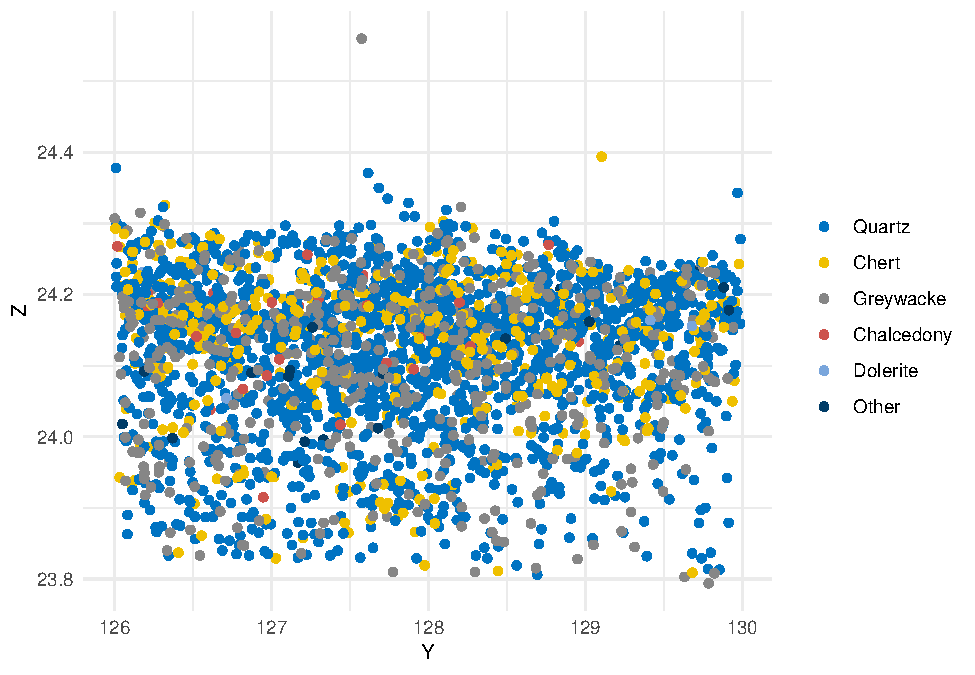
\includegraphics{thesis_files/figure-latex/spatialdistributionVB-1.pdf}
\caption{\label{fig:spatialdistributionVB}Spatial distribution of lithic artefacts (without chips) by raw material, on unit H.}
\end{figure}
However, when calculating the percentages of the three most important raw materials by cubic meter of excavated sediment (Figure \ref{fig:rmdispersion}) and plotting them by depth, there are significant differences in raw material distribution over time. From around 24.1 m of depth upwards, there is an important shift in quartz and chert frequencies, the latter increasing more than 10\%, and quartz dropping from c.~50\% to nearly 30\%. Greywacke frequencies follow those of quartz.

This shift seems to be associated with other significant changes in the Terrace sequence, such as the abovementioned increase in the amount of lithic materials in top Layer 5 and Layer 4E, but also the appearance of Vale Comprido technology (fig.~\ref{fig:spatialvbfig}). Additionally, these two moments are stratigraphically correlated with two different chronological horizons, the first, dated to c.~26 kcal BP, at c.~23.9 m depth, and associated with higher frequencies of quartz, and the second, dated to c.~24.7 kcal BP, at around 24.1 m depth, associated with higher frequencies of chert and a reduction in quartz presence.
\begin{verbatim}
`geom_smooth()` using method = 'loess' and formula 'y ~ x'
\end{verbatim}
\begin{figure}
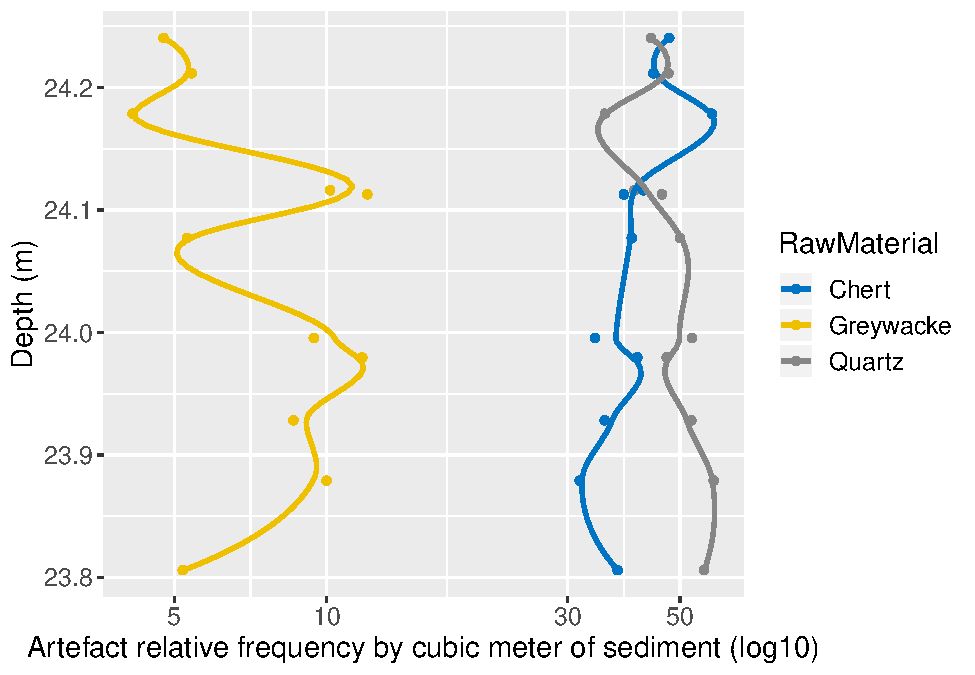
\includegraphics[width=1\linewidth]{thesis_files/figure-latex/rmdispersion-1} \caption{Raw material discard rates over time at Vale Boi. Each point is an excavation unit (spit). The lines are locally weighted regression lines (span ¼ 0.4) to aid in visualising the trend of increased discard in the upper part of the deposit.}\label{fig:rmdispersion}
\end{figure}
As such, and given the chronological, density of artifacts, and raw material preference patterns, it was decided that for this study the materials would be subdivided in two analytical units, to better understand any possible technological differences: \emph{Lower 5}, including all artifacts with Z values under 24.1; \emph{Upper 5/4E}, including all artifacts with Z values of 24.1 and above. The value 24.1 is arbitrary and was chosen for the reasons aforementioned: it seems to be where the separation between higher and lower densities of lithic materials occurs and, also, where the inversion of quartz and chert frequencies happens.

A total of 26703 pieces were analyzed for both groups, 11094 from Lower 5 group (table \ref{tab:general1}) and 15609 for the Upper 5/4E (table \ref{tab:general2}). Most of these are chips (70.62\% from Lower 5 and 65.68\% from Upper 5/4E), followed by shatters, which make up c.~21\% and c.~24\% of the groups, respectively. These extremely high numbers for debris are mostly the result of quartz use, which can be explained not only by on-site knapping of this raw material but mostly by its breakage patterns (especially when coarser), which typically produces more waste than in other raw materials.

For Lower 5, cores and debitage products represent a cumulative frequency of c.~8\%. For Upper 5/4E, debitage products represent nearly 10\% of the group's assemblage. Complete blanks are the most represented class for both groups, with 1474 identified pieces, 4.59\% for Lower 5 and 6.18\% for Upper 5/4E, followed by blank fragments, with an absolute count of 248 for Lower 5 and 336 for Upper 5/4E. Cores are also relatively frequent within these assemblages, with an absolute count of 123 cores, 46 for Lower 5 and 77 for Upper 5/4E, while core fragments appear in much smaller numbers (n=11 and n=14, respectively).

During the analysis, 167 retouched pieces were identified, 55 on Lower 5, representing 0.5\% of the group, and 112 on Upper 5/4E, with a frequency of 0.72\%. Retouched piece fragments composed a much smaller number (n = 7 for Lower 5 and n = 16 for Upper 5/4E).
\begin{landscape}\begin{table}

\caption{\label{tab:general1}Technological class by raw material for Lower 5.}
\centering
\resizebox{\linewidth}{!}{
\begin{tabular}[t]{>{\bfseries}lrlrlrlrlrlrlrl}
\toprule
Class & Quartz (n) & Quartz (\%) & Chert (n) & Chert (\%) & Greywacke (n) & Greywacke (\%) & Dolerite (n) & Dolerite (\%) & Chalcedony (n) & Chalcedony (\%) & Other (n) & Other (\%) & Total & Total (\%)\\
\midrule
Anvil & 0 & 0\% & 0 & 0\% & 2 & 0.09\% & 0 & 0\% & 0 & 0\% & 0 & 0\% & 2 & 0.02\%\\
Blank & 281 & 3.58\% & 171 & 15.86\% & 44 & 2.08\% & 3 & 50\% & 6 & 37.5\% & 4 & 11.76\% & 509 & 4.59\%\\
BlankFrag & 132 & 1.68\% & 90 & 8.35\% & 23 & 1.09\% & 1 & 16.67\% & 1 & 6.25\% & 1 & 2.94\% & 248 & 2.24\%\\
Core & 18 & 0.23\% & 23 & 2.13\% & 3 & 0.14\% & 0 & 0\% & 1 & 6.25\% & 1 & 2.94\% & 46 & 0.41\%\\
CoreFrag & 2 & 0.03\% & 8 & 0.74\% & 0 & 0\% & 1 & 16.67\% & 0 & 0\% & 0 & 0\% & 11 & 0.1\%\\
\addlinespace
CorePreparProd & 1 & 0.01\% & 0 & 0\% & 0 & 0\% & 0 & 0\% & 0 & 0\% & 0 & 0\% & 1 & 0.01\%\\
Manuport & 0 & 0\% & 0 & 0\% & 2 & 0.09\% & 0 & 0\% & 0 & 0\% & 1 & 2.94\% & 3 & 0.03\%\\
RetouchedPiece & 15 & 0.19\% & 38 & 3.53\% & 1 & 0.05\% & 0 & 0\% & 1 & 6.25\% & 0 & 0\% & 55 & 0.5\%\\
RetouchedPieceFrag & 3 & 0.04\% & 4 & 0.37\% & 0 & 0\% & 0 & 0\% & 0 & 0\% & 0 & 0\% & 7 & 0.06\%\\
Shatter & 1754 & 22.36\% & 95 & 8.81\% & 507 & 23.96\% & 0 & 0\% & 5 & 31.25\% & 16 & 47.06\% & 2377 & 21.43\%\\
\addlinespace
Chip & 5638 & 71.88\% & 649 & 60.2\% & 1534 & 72.5\% & 1 & 16.67\% & 2 & 12.5\% & 11 & 32.35\% & 7835 & 70.62\%\\
Total & 7844 & - & 1078 & - & 2116 & - & 6 & - & 16 & - & 34 & - & 11094 & -\\
\bottomrule
\end{tabular}}
\end{table}
\end{landscape}
\begin{landscape}\begin{table}

\caption{\label{tab:general2}Technological class by raw material for Upper 5/4E.}
\centering
\resizebox{\linewidth}{!}{
\begin{tabular}[t]{>{\bfseries}lrlrlrlrlrlrlrl}
\toprule
Class & Quartz (n) & Quartz (\%) & Chert (n) & Chert (\%) & Greywacke (n) & Greywacke (\%) & Dolerite (n) & Dolerite (\%) & Chalcedony (n) & Chalcedony (\%) & Other (n) & Other (\%) & Total & Total (\%)\\
\midrule
Blank & 438 & 3.91\% & 407 & 19.53\% & 80 & 3.62\% & 14 & 60.87\% & 18 & 32.14\% & 8 & 34.78\% & 965 & 6.18\%\\
BlankFrag & 151 & 1.35\% & 155 & 7.44\% & 20 & 0.9\% & 3 & 13.04\% & 7 & 12.5\% & 0 & 0\% & 336 & 2.15\%\\
Burin spall & 0 & 0\% & 1 & 0.05\% & 0 & 0\% & 0 & 0\% & 0 & 0\% & 0 & 0\% & 1 & 0.01\%\\
Core & 32 & 0.29\% & 42 & 2.02\% & 1 & 0.05\% & 0 & 0\% & 0 & 0\% & 2 & 8.7\% & 77 & 0.49\%\\
CoreFrag & 4 & 0.04\% & 10 & 0.48\% & 0 & 0\% & 0 & 0\% & 0 & 0\% & 0 & 0\% & 14 & 0.09\%\\
\addlinespace
CorePreparProd & 1 & 0.01\% & 5 & 0.24\% & 0 & 0\% & 0 & 0\% & 0 & 0\% & 0 & 0\% & 6 & 0.04\%\\
Manuport & 0 & 0\% & 0 & 0\% & 5 & 0.23\% & 0 & 0\% & 0 & 0\% & 1 & 4.35\% & 6 & 0.04\%\\
RetouchedPiece & 34 & 0.3\% & 70 & 3.36\% & 2 & 0.09\% & 5 & 21.74\% & 1 & 1.79\% & 0 & 0\% & 112 & 0.72\%\\
RetouchedPieceFrag & 6 & 0.05\% & 9 & 0.43\% & 1 & 0.05\% & 0 & 0\% & 0 & 0\% & 0 & 0\% & 16 & 0.1\%\\
Shatter & 3006 & 26.81\% & 227 & 10.89\% & 563 & 25.46\% & 1 & 4.35\% & 15 & 26.79\% & 12 & 52.17\% & 3824 & 24.5\%\\
\addlinespace
Chip & 7540 & 67.25\% & 1158 & 55.57\% & 1539 & 69.61\% & 0 & 0\% & 15 & 26.79\% & 0 & 0\% & 10252 & 65.68\%\\
Total & 11212 & - & 2084 & - & 2211 & - & 23 & - & 56 & - & 23 & - & 15609 & -\\
\bottomrule
\end{tabular}}
\end{table}
\end{landscape}
\hypertarget{lapa-do-picareiro-2}{%
\subsection{Lapa do Picareiro}\label{lapa-do-picareiro-2}}

The materials from Lapa do Picareiro selected for this study come exclusively from Levels U and T. Based on chronological data and artifact distribution along the sequence, these levels had been previously organized into two distinct cultural horizons (Haws et al., 2019), somehow similar to the Terminal Gravettian and Proto-Solutrean phases in the traditional transition model (Zilhão, 1997; Zilhão, Aubry, \& Almeida, 1999).

Given this geo-archaeological background, for the present analysis the materials were separated into two assemblages: \emph{U/Lower T}, which included all artifacts with depths inferior to 566.9 m or (in case of artifacts lacking 3D coordinates) from all spits from Level U and spits 6 through 8 from Level T (Haws et al., 2019); \emph{Middle T}, including all artifacts with depths equal or superior to 566.9 m, or from the top five spits of Level T. Any other artifact in the assemblage which did not have a depth value or Level/Spit was not considered in these results since it lacked the needed information to contextualize its technological attributes. Also excluded from this study are the materials found on top of Level T, undoubtedly attributeable to the solutrean (Benedetti, Haws, Bicho, Friedl, \& Ellwood, 2019; Haws et al., 2019).

A total of 376 pieces were analyzed, 196 coming from the U/Lower T phase and 180 from the Middle T group. In both groups, debitage waste is mostly composed of chips, which represents 49.5\% of the U/Lower T group and 37.2\% of the Middle T group. As in Vale Boi, these values for chippage can be mostly explained by quartz breakage patterns.

The second most present class for both assemblages are complete blanks, which represent 13.7\% of the U/Lower T group and 37.2\% of the Middle T group, followed by blank fragments (13.7\% and 15.5\%, respectively). Retouched pieces have relatively small frequencies, representing c.~3\% in both U/Lower T and Middle T. Cores are very scarce in both groups, 1\% in the U/Lower T group (n=2) and c.~3\% in the Middle T (n=5).
\begin{table}

\caption{\label{tab:general1lp}Technological class by raw material (U/Lower T phase).}
\centering
\resizebox{\linewidth}{!}{
\begin{tabular}[t]{>{\bfseries}lrlrlrlrl}
\toprule
Class & Quartz (n) & Quartz (\%) & Chert (n) & Chert (\%) & Other (n) & Other (\%) & Total & Total (\%)\\
\midrule
Blank & 30 & 20.83\% & 24 & 53.33\% & 1 & 14.29\% & 55 & 28.06\%\\
BlankFrag & 22 & 15.28\% & 4 & 8.89\% & 1 & 14.29\% & 27 & 13.78\%\\
Core & 2 & 1.39\% & 0 & 0\% & 0 & 0\% & 2 & 1.02\%\\
CorePreparProd & 0 & 0\% & 1 & 2.22\% & 0 & 0\% & 1 & 0.51\%\\
Manuport & 0 & 0\% & 0 & 0\% & 1 & 14.29\% & 1 & 0.51\%\\
\addlinespace
RetouchedPiece & 1 & 0.69\% & 5 & 11.11\% & 0 & 0\% & 6 & 3.06\%\\
Shatter & 4 & 2.78\% & 1 & 2.22\% & 2 & 28.57\% & 7 & 3.57\%\\
Chip & 85 & 59.03\% & 10 & 22.22\% & 2 & 28.57\% & 97 & 49.49\%\\
Total (RM) & 144 & - & 45 & - & 7 & - & 196 & -\\
\bottomrule
\end{tabular}}
\end{table}
\begin{table}

\caption{\label{tab:general2lp}Technological class by raw material (Middle T phase).}
\centering
\resizebox{\linewidth}{!}{
\begin{tabular}[t]{>{\bfseries}lrlrlrlrl}
\toprule
Class & Quartz (n) & Quartz (\%) & Chert (n) & Chert (\%) & Other (n) & Other (\%) & Total & Total (\%)\\
\midrule
Blank & 19 & 19\% & 46 & 63.01\% & 2 & 28.57\% & 67 & 37.22\%\\
BlankFrag & 19 & 19\% & 9 & 12.33\% & 0 & 0\% & 28 & 15.56\%\\
Core & 2 & 2\% & 2 & 2.74\% & 1 & 14.29\% & 5 & 2.78\%\\
RetouchedPiece & 0 & 0\% & 5 & 6.85\% & 0 & 0\% & 5 & 2.78\%\\
Shatter & 3 & 3\% & 2 & 2.74\% & 3 & 42.86\% & 8 & 4.44\%\\
\addlinespace
Chip & 57 & 57\% & 9 & 12.33\% & 1 & 14.29\% & 67 & 37.22\%\\
Total (RM) & 100 & - & 73 & - & 7 & - & 180 & -\\
\bottomrule
\end{tabular}}
\end{table}
\hypertarget{raw-materials}{%
\section{Raw materials}\label{raw-materials}}

Raw material use and availability, specifically abundance and quality, stand as important factors for understanding the organization of technology, as it may affect decisions regarding tool design and conservation of such tools (Andrefsky, 1994), as well as mobility and niche expansion (J. M. M. Cascalheira, 2013). This quality is connected to both the raw material's fracture mechanics and their intrinsic mineral characteristics, such as the size of their grain, homogeneity (Andrefsky, 1994), or even hardness (Kempson \& Wadley, 2011), which allow the knapper predictability over the outcome (Andrefsky, 2005).

There are a number of stones that are constant throughout the stone age archaeological record for having the necessary properties described above. Stones or minerals characterized by high frequencies of silica, such as chert or quartz, allow for good fracture predictability, while other materials with less homogeneity may progressively result in less predictable characteristics (Andrefsky, 2005). Thus, despite the raw material variability within the pre-historic archaeological record, linked to its availability and geomorphological contexts of the sites, the selection is often coherent regarding fracture mechanics, where predictable conchoidal fractures are preferred (Andrefsky, 2005; Inizan, Reduron-Ballinger, Roche, \& Tixier, 1999; Tixier \& Inizian, 1980).

This pattern is also observable at Vale Boi and Lapa do Picareiro as shown below. Previous studies have shown that throughout most levels of human occupation at both sites, chert, fine quartz and greywacke (the latter in the case of Vale Boi only) or quartzite (in the case of Lapa do Picareiro) (all three characterized by conchoidal fracture, although greywacke and quartzite are often coarse and more unpredictable) were the most frequently used (Benedetti et al., 2019; Bicho, Cascalheira, \& Marreiros, 2012; Cascalheira, 2010; Haws et al., 2019; Marreiros, 2009; Pereira et al., 2016). While at Vale Boi all the materials are available at a regional and local scale, at Lapa do Picareiro a more detailed analysis is needed to assess raw material provenance. Also, although the presence of the main raw materials is documented across all archaeological levels in Vale Boi, with each occupation differing in the frequency of their use, chert is always the primary material used for knapping (Cascalheira, 2010). At Lapa do Picareiro, the use of chert is not always a preference, such as in the case of Level FF, where quartzite is clearly dominant. The characteristics of Lapa do Picareiro and the potential functional specificities of each occupation must have had a significant impact on the type and quality of the discard materials.

For the present study, criteria used for raw material analysis focused on the identification of broader groups of stones and minerals, based on their general observable characteristics, without focusing on particular features within each raw material. Two exceptions were made, however. At both sites, quartz was subdivided into different categories regarding the size of the grain, to isolate and better understand the different uses of quartz over time. At Lapa do Picareiro, chert was organized based on color to evaluate the integrity of the deposits and, preliminarly, explore the spatial organization of levels U and T. Both of these exceptions are presented in the following sections where the patterns of exploitation of the more relevant raw materials are discussed for each site.

\hypertarget{vale-boi-3}{%
\subsection{Vale Boi}\label{vale-boi-3}}

One of the most relevant raw materials in both of Vale Boi analytical units used for this study is quartz (encompassing rock crystal, fine, medium and coarse qualities), which represents c.~43\% of the total assemblage for the Upper 5/4E group, and c.~51\% for Lower 5. Chert, on the other hand, represents c.~46\% of the Upper 5/4E phase and 38\% of the Lower 5. Finally, greywacke, dolerite, chalcedony, and other raw materials that due to their low frequencies were collapsed in the category ``Other'', together represent c.~11\% of both assemblages (Figure \ref{fig:rmvb}).
\begin{figure}
\centering
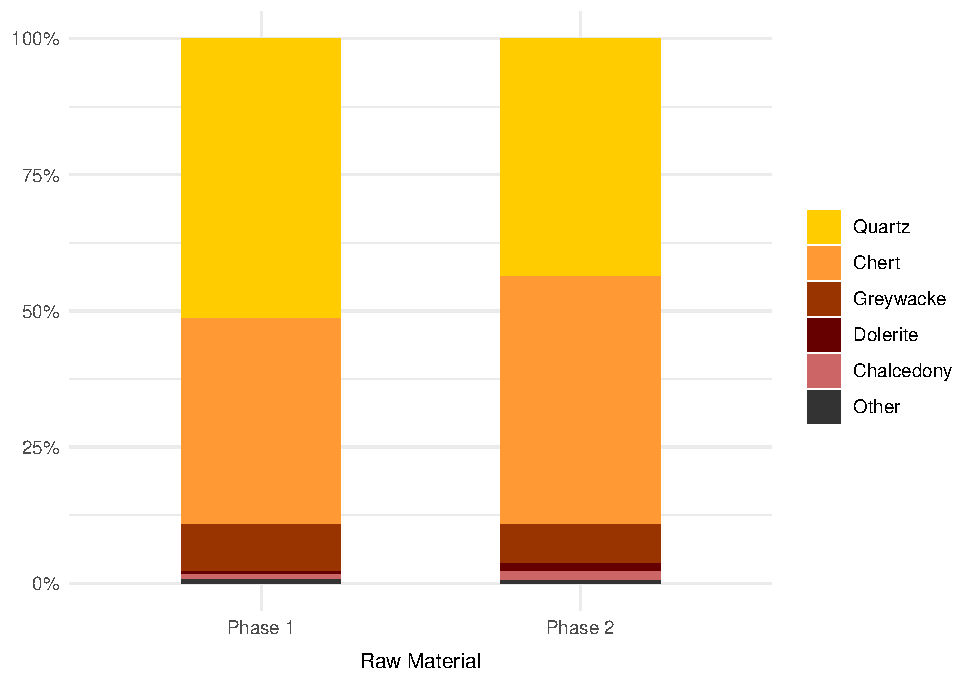
\includegraphics{thesis_files/figure-latex/rmvb-1.pdf}
\caption{\label{fig:rmvb}Vale Boi. Frequencies of raw materials by phase. Chips and shatters not included.}
\end{figure}
\hypertarget{quartz}{%
\subsubsection{Quartz}\label{quartz}}

The number of chips and shatter in quartz are, as seen in tables \ref{tab:general1} and \ref{tab:general2}, extremely high, both in its representativity within the raw material, with c.~94\% for both Lower 5 and Upper 5/4E, and when compared to the relative frequencies of other raw materials.

Despite the low frequencies presented on the table, there is a large number of quartz blanks (n=281 for Lower 5 and n=438 for Upper 5/4E) compared to the rest of the classes, as well as cores (n=18 for Lower 5 and n=32 for Upper 5/4E) and retouched pieces (n=15 for Lower 5 and n=34 for Upper 5/4E).
Most of the quartz artifacts do not show the presence of cortex, with nearly 95\% of all artifacts having 0\% cortex (Figure \ref{fig:rmcortex}). When cortex is present, around 72\% of the artifacts indicate the exploitation of cobbles or pebbles. These patterns are similar for both Lower 5 and Upper 5/4E (table \ref{tab:cortextab1}).

As mentioned before, quartz was organized into groups regarding grain size. Analyzing the artifact class frequency through the different identified types of quartz confirmed an already expected pattern: the production of blanks was largely accomplished using fine and medium quality quartz (52.1\% and 32.7\% for Lower 5, table \ref{tab:quartzquality1} and 49.3\% and 32.1\% for Upper 5/4E, table \ref{tab:quartzquality2}, respectively). Most of the retouched tools were also recorded for these two types of quartz quality (66.7\% and 26.7\% for Lower 5, and 55.9\% and 44.1\% for Upper 5/4E). No retouched pieces were identified in coarse quartz and rock crystal. The latter type represents, also, a rather small fraction of the assemblage. In accordance with previous studies on Vale Boi lithic industries (e.g.~Cascalheira 2009, Marreiros 2009) coarse quartz appears mostly as knapping shatters, or as other type of fragments not related to human knapping (see Manne et al.~2012 for more information).
\begin{table}

\caption{\label{tab:quartzquality1}Vale Boi - Lower 5. Frequencies of technological classes by quartz quality.}
\centering
\resizebox{\linewidth}{!}{
\begin{tabular}[t]{>{\bfseries}llllll}
\toprule
Quartz quality & Blank & Core & CorePreparProd & RetouchedPiece & Total\\
\midrule
QuartzQuality, n (\%) &  &  &  &  & \\
Coarse & 40 (14.2) & 5 (27.8) & 0 (0.0) & 1 (6.7) & 46 (14.6)\\
Fine & 148 (52.7) & 6 (33.3) & 0 (0.0) & 10 (66.7) & 164 (52.1)\\
Medium & 91 (32.4) & 7 (38.9) & 1 (100.0) & 4 (26.7) & 103 (32.7)\\
RockCrystal & 2 (0.7) & 0 (0.0) & 0 (0.0) & 0 (0.0) & 2 (0.6)\\
\bottomrule
\end{tabular}}
\end{table}
\begin{table}

\caption{\label{tab:quartzquality2}Vale Boi - Upper 5/4E. Frequencies of technological classes by quartz quality.}
\centering
\resizebox{\linewidth}{!}{
\begin{tabular}[t]{>{\bfseries}llllll}
\toprule
Quartz quality & Blank & Core & CorePreparProd & RetouchedPiece & Total\\
\midrule
QuartzQuality, n (\%) &  &  &  &  & \\
Coarse & 82 (18.7) & 9 (28.1) & 0 (0.0) & 0 (0.0) & 91 (18.0)\\
Fine & 223 (50.9) & 7 (21.9) & 0 (0.0) & 19 (55.9) & 249 (49.3)\\
Medium & 130 (29.7) & 16 (50.0) & 1 (100.0) & 15 (44.1) & 162 (32.1)\\
RockCrystal & 3 (0.7) & 0 (0.0) & 0 (0.0) & 0 (0.0) & 3 (0.6)\\
\bottomrule
\end{tabular}}
\end{table}
\hypertarget{chert}{%
\subsubsection{Chert}\label{chert}}

Chert shows high frequencies of blanks (15.8\% for Lower 5 and 19.6\% for Upper 5/4E) when compared to every other class, excluding chips (tables \ref{tab:general1} and \ref{tab:general2}). The latter represents more than 50\% of the chert assemblages, with an absolute frequency of 649 chips for Lower 5 and 1158 for Upper 5/4E.

Although chert shows smaller absolute numbers for blanks (n=171 for Lower 5 and n=407 for Upper 5/4E) and blank fragments (n=90 for Lower 5 and n=155 for Upper 5/4E) compared to quartz, there is a large quantity of cores representing 2.1\% of total chert in Lower 5 and 2\% in Upper 5/4E. However, tables \ref{tab:general1} and \ref{tab:general2} show a noticeable difference in the ratio between chert blanks and quartz blanks in Lower 5 and Upper 5/4E, with the latter showing a higher frequency of chert blanks compared to Upper 5/4E.

Regarding retouched pieces, these represent more than 3\% of chert for both phases, a number far higher than those in other raw materials. This shows that chert, although less present than quartz in blank absolute count (although barely in Upper 5/4E), might have been preferentially used for formal tool production.

Chert also shows the most prominent variability of cortex frequencies in both phases (Figure @(fig:rmcortex)), although there is a clear dominance of artifacts with 0\% cortex, a pattern that was already expected, following the process of the knapping sequence, where only the first blanks removed from an unmodified block will be entirely cortical, showing increasingly less cortex for posterior removals (Andrefsky, 2005). It is noteworthy, however, that for both phases, a significant number of chert artifacts (c.~25\%) presented cortical surfaces, confirming that chert nodules were imported to the site and thus all phases of the reduction sequences are likely represented.

This variability in cortex presence is accompanied by some diversity of cortex types, with the presence of both cobble and outcrop sources, even though for almost 85\% of the artifacts it was not possible to identify a specific type of cortex (Table \ref{tab:cortextab1}).

\hypertarget{greywacke}{%
\subsubsection{Greywacke}\label{greywacke}}

Greywacke is a variety of sandstone, often characterized by its hardness, dark color and poorly sorted grains of quartz and feldspar (Haldar, 2013). At Vale Boi, this raw material is highly heterogeneous, showing a wide variety of grain sizes and colors.

Within the studied assemblage, greywacke is best represented by debitage waste, with around 25\% of shatter and 70\% of chips, for both Lower 5 and Upper 5/4E. In contrast, relatively low numbers for blanks (n=44 for Lower 5 and n=80 for Upper 5/4E) and cores (n=3 for Lower 5 and 1 for Upper 5/4E) were recorded. The same applies to the retouched tools category, with three artifacts recorded, one of which is a Vale Comprido piece, in the Upper 5/4E phase.

When chips and shatters are removed, greywacke has a representation of less than 10\% in both assemblages making it the third most used raw material (figure \ref{fig:rmvb}).

Similarly to the other raw materials, there is, for both phases, the predominance of debitage without cortex (Figure \ref{fig:rmcortex}). There is, however, some variability in cortex presence, even if in smaller frequencies than the patterns observed for chert. As in the case of quartz, most of the identified cortex presented water-worned surfaces, indicating the exploitation of cobbles or, most likely, slabs.

\hypertarget{dolerite}{%
\subsubsection{Dolerite}\label{dolerite}}

Dolerite is a volcanic igneous rock, occurring mostly in dikes, varying between coarse and fine textures, and often having a dark, grey or greyish-green coloration (Haldar, 2013; Kempson \& Wadley, 2011). Its presence is registered in the Algarve, through occasional outcrops and infiltrations in the southwest regions of the Algarve (Oliveira, 1984), also appearing as outcrops within the Messejana fault (Belmiro, 2018).

At Vale Boi, this raw material was first identified as jasper when excavating the levels referring to the proto-solutrean occupation in the Terrace area (units J-L), before 2012 (Marreiros, 2009). The material has a very characteristic reddish-brown color and fine texture, with a conchoidal fracture. Despite this coloration, which is also present in jasper (a red-colored variety of chalcedony), the raw material was later identified as dolerite, and its coloration explained by the presence of a reddish patina which would have altered the original rock by processes of iron mineral oxidation through contact with the terra rossa (Belmiro, 2018).

The analysis of a thin section obtained from a dolerite fragment from the present assemblage allowed the characterization of this raw material, through its visible features and petrography.

The reddish coloration was confirmed to be an exterior patina, no more than 1 mm thick, completely covering the artifacts. The actual rock still displays a fine texture but with an opaque black color.

Results from the petrographic analysis done through the observation of the thin section using a polarizing microscope revealed the presence of several minerals, such as feldspar, plagioclase, quartz, small quantities of silica, little presence of mica and iron oxide, which are in concordance with the mineral composition of dolerite or possibly hornfels (Kempson \& Wadley, 2011). The feldspar minerals showed the presence of undulatory extinction, a deformation that takes place whenever certain minerals are exposed to high temperatures (Frost \& Frost, 2019), thus indicating that the raw material is highly metamorphized.

Regarding the differentiation between dolerite and hornfels, although these two rocks have different origins, the latter being of volcanic igneous origin, considered a contact metamorphic rock (Haldar, 2013), they share enough visual and mineral characteristics (whenever the dolerite has a fine texture) to hinder their precise identification. Literature most often uses other methods to differentiate them, such as FTIR or XRF, by understanding not the mineral composition (which is essentially the same) but the ratio of components presence. This matter is further complexified by understanding that hornfels might originate from metamorphized igneous rocks, several sources of hornfels attributed to dolerite dikes (Hallinan \& Shaw, 2015; Kempson \& Wadley, 2011).

Given this difficulty, although the present analysis will use the term dolerite, for their reported similarities in terms of texture, grain size and fracture, further chemical studies need to be done in order to confirm whether the raw material is dolerite or possibly hornfels. Regarding the latter, there is also the presence of hornfels outcrops and rounded pebbles in the Algarve, near the southwestern coast, thus strengthening the hypothesis that this raw material, whether dolerite or hornfels, is available regionally.

Looking at the interior of dolerite allowed, during the second moment of analysis, to identify other products in the same raw material, which were not previously identified due to the lack of the same reddish patina. This patina also appears throughout the assemblage, mostly on greywacke, although without forming the same 1 mm thick layer visible on the dolerite pieces. This may be explained by the inherent mineral characteristics of this type of raw material and their reaction with the surrounding sediment.

The presence of this patina in several degrees of intensity, preferentially in dolerite and greywacke, its presence in both finished complete artifacts and flake fragments or shatters, and its occurrence also reported in the literature as a process frequently affecting raw materials like hornfels (e.g., Hallinan and Shaw 2015), suggests that it is, in fact, the result of geological and chemical processes affecting these raw materials. Its absence from other raw materials, like chert or quartz, may reflect the inherent mineral properties of these rocks.

Dolerite is a rather unusual raw material in the site of Vale Boi, appearing only in layers 4E and 5 of the Terrace and proto-solutrean levels of the Slope area. The most striking characteristic of this raw material in the assemblages under study is the low presence of chips or shatter (n=1 each), but high frequencies of blanks (50\% in Lower 5 and 60.8\% in Upper 5/4E) and blank fragments (16.6\% in Lower 5 and 13\% in Upper 5/4E) (tables \ref{tab:general1} and \ref{tab:general2}). Unlike Lower 5, in Upper 5/4E dolerite is represented by five retouched tools, some of which are Vale Comprido points. This raw material seems to have been used preferentially at Vale Boi for the production of these types of points, a pattern already observed in previous works (Marreiros, 2009), where three out of five Vale Comprido points were identified as dolerite (originally jasper).

The absence of cores, with only one core fragment identified in the Lower 5 group, and low quantity of debitage waste may be explained by the importation of finished pieces or blanks to the site, suggesting that, most likely, no knapping activities occurred with this raw material at the site. This interpretation is, however, truncated by this study's phase analysis. As the identification of the inner aspect of dolerite was only achieved at the start of the second phase, which as referred before, consisted of the analysis of all cores and debitage products with a more complete database, shatter, chips and fragments were not revisited, thus not allowing for the possible identification of unpatinated dolerite within those classes, which might have been mistaken for fine-grained greywacke. This caveat does not, however, seem to influence the patterns regarding complete blank and retouched tools frequency.

\hypertarget{chalcedony}{%
\subsubsection{Chalcedony}\label{chalcedony}}

Chalcedony is a type of cryptocrystalline quartz, characterized by a waxy and glossy appearance, ranging from a variety of possible colors (Haldar, 2013), although white is the only present variety in the studied assemblages. The chalcedony in levels 5 and 4E is also characterized by the frequent presence of inclusions, making this raw material poorly homogeneous.

Results indicate it may have been mainly used for the production of blanks, which represent 37.5\% of chalcedony in Lower 5 (table \ref{tab:general1}) and 32.1\% in Upper 5/4E (table \ref{tab:general2}), with a rather small representation of retouched pieces (n=2), which include a Vale Comprido point in the Upper 5/4E group. The presence of a core in Lower 5, as well as the presence of shatter and chips (in small numbers, n\textless5 each for Lower 5 and n=15 each for Upper 5/4E, respectively) may indicate, contrary to the dolerite, onsite knapping of this raw material.

Compared to other raw materials, chalcedony has the lowest frequencies of cortex, in both phases, with almost 100\% of all artifacts (except shatter and chips) having 0\% cortex (Figure \ref{fig:rmcortex}).
\begin{figure}
\centering
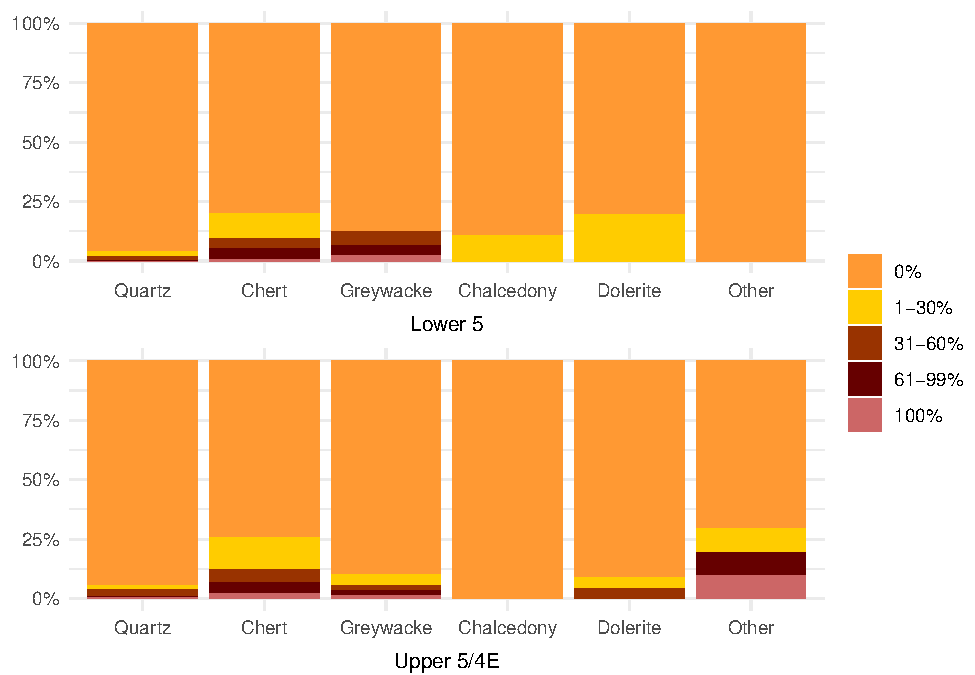
\includegraphics{thesis_files/figure-latex/rmcortex-1.pdf}
\caption{\label{fig:rmcortex}Vale Boi. Frequencies of cortex by raw material and phase. Chips and shatters not included.}
\end{figure}
\begin{table}

\caption{\label{tab:cortextab1}Vale Boi - Lower 5. Frequencies of cortex type by raw material.}
\centering
\resizebox{\linewidth}{!}{
\begin{tabular}[t]{>{\bfseries}lllll}
\toprule
Cortex attributes & Quartz & Chert & Greywacke & Total\\
\midrule
CortexType, n (\%) &  &  &  & \\
Cobble & 15 (83.3) & 5 (8.5) & 7 (77.8) & 27 (31.0)\\
Indeterminate & 2 (11.1) & 50 (84.7) & 0 (0.0) & 53 (60.9)\\
Outcrop & 1 (5.6) & 4 (6.8) & 2 (22.2) & 7 (8.0)\\
\bottomrule
\end{tabular}}
\end{table}
\begin{table}

\caption{\label{tab:cortextab2}Vale Boi - Upper 5/4E. Frequencies of cortex typeby raw material.}
\centering
\begin{tabular}[t]{>{\bfseries}lllllll}
\toprule
Cortex attributes & Quartz & Chert & Greywacke & Dolerite & Other & Total\\
\midrule
CortexType, n (\%) &  &  &  &  &  & \\
Cobble & 30 (81.1) & 11 (6.7) & 9 (81.8) & 2 (100.0) & 3 (100.0) & 55 (25.3)\\
Indeterminate & 4 (10.8) & 123 (75.0) & 2 (18.2) & 0 (0.0) & 0 (0.0) & 129 (59.4)\\
Outcrop & 3 (8.1) & 30 (18.3) & 0 (0.0) & 0 (0.0) & 0 (0.0) & 33 (15.2)\\
\bottomrule
\end{tabular}
\end{table}
\hypertarget{lapa-do-picareiro-3}{%
\subsection{Lapa do Picareiro}\label{lapa-do-picareiro-3}}

Comparatively to Vale Boi, Lapa do Picareiro shows less raw material variability, which might be explained by the lithological characteristics of the area, already explored in other studies that showed similar raw material presence patterns (Almeida, 2000; Zilhão, 1997), but can also be related to the location of the site in a high altitude environment with significant implications to the functional nature of the occupations (see Cascalheira and Bicho 2017). The main raw materials identified were quartz and chert (Figure \ref{fig:rmlp}). Quartz is dominant in the U/Lower T phase, representing c.~60\% of the assemblage, while chert is dominant in the Middle T phase, representing c.~59\%. The sporadic occurrence of other raw materials is the result of the identification of some quartzite artifacts on both phases.
\begin{figure}
\centering
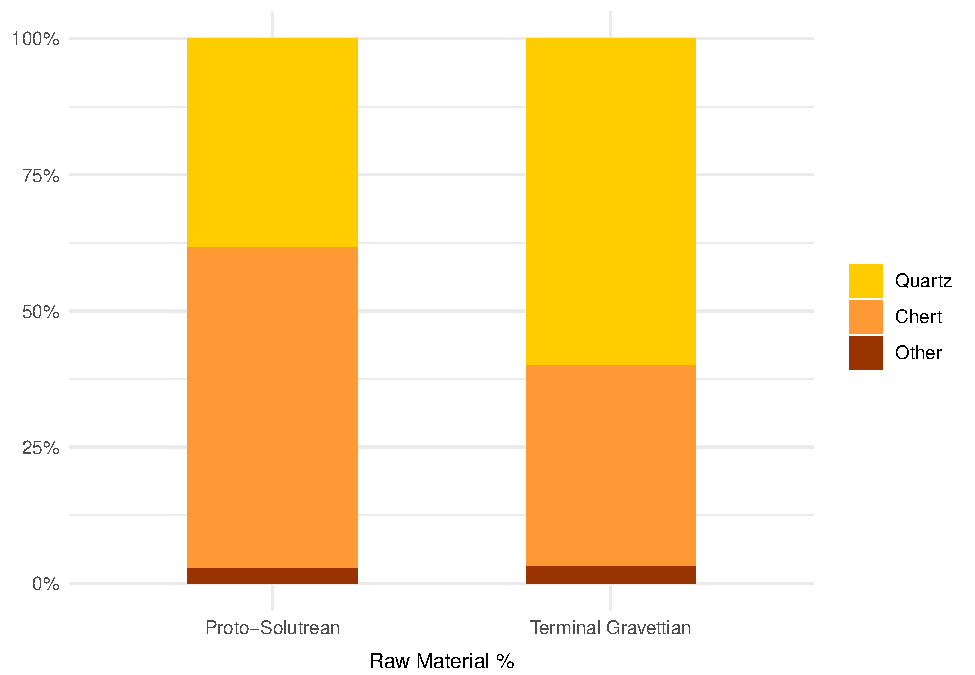
\includegraphics{thesis_files/figure-latex/rmlp-1.pdf}
\caption{\label{fig:rmlp}Lapa do Picareiro. Frequencies of raw material by phase. Chips and shatters not included.}
\end{figure}
\hypertarget{quartz-1}{%
\subsubsection{Quartz}\label{quartz-1}}

The number of chips in quartz, as seen on tables \ref{tab:general1LP} and \ref{tab:general2LP}, is extremely high, representing nearly 60\% of this raw material in both phases. Other waste products, i.e.~shatters, show much smaller numbers (n=4 for U/Lower T and n=3 for Middle T). Comparatively, complete blanks are the second most present class in quartz, with a frequency of 20\% (n=30) for the U/Lower T group, followed by blank fragments which represent 15.2\% of that assemblage. For the Middle T group, complete blanks and blank fragments show similar frequencies, representing c.~19\% each. Although in small numbers, quartz shows the highest number of cores (n=4, 2 in each group) from all raw materials, but a small number of retouched tools (n=1).

Regarding cortex, quartz shows frequencies as low as 6\% for cortex presence on the U/Lower T group, 12.5\% on the Middle T, being mostly composed of pieces with no cortex on their dorsal surfaces. When present, cortical surfaces are all water-worned, indicating the exploitation of cobbles/pebbles (Tables \ref{Tab:cortextabtg} and \ref{tab:cortextabpr}).

As in Vale Boi, quartz was categorized regarding grain quality and color (Tables @ref(tab:quartzqualityTG and \ref{tab:quartzqualityPR}. For both the U/Lower T group and Middle T, it is possible to observe a majority of fine quality quartz and rock crystal for both cores and blanks, with barely any presence of medium and coarse quality quartz. The latter category is completely absent in the Middle T group.

One observable difference between the two groups is in the percentages of rock crystal and fine quality: in the U/Lower T, fine quality quartz represents c.~56\% of quartz, while rock crystal has a frequency of nearly 41\%; for Middle T, these percentages change, as fine quality quartz represents c.~38\%, against c.~57\% of rock crystal. Finally, the single identified retouched tool in U/Lower T was made in fine quality quartz.
\begin{table}

\caption{\label{tab:quartzqualityTG}Lapa do Picareiro - U/Lower T. Frequencies of technological classes by quartz quality.}
\centering
\begin{tabular}[t]{>{\bfseries}lllll}
\toprule
Quartz quality & Blank & Core & RetouchedPiece & Total\\
\midrule
QuartzQuality, n (\%) &  &  &  & \\
Fine & 16 (53.3) & 1 (50.0) & 1 (100.0) & 30 (54.5)\\
Medium & 1 (3.3) & 0 (0.0) & 0 (0.0) & 1 (1.8)\\
RockCrystal & 13 (43.3) & 1 (50.0) & 0 (0.0) & 24 (43.6)\\
\bottomrule
\end{tabular}
\end{table}
\begin{table}

\caption{\label{tab:quartzqualityPR}Lapa do Picareiro - Middle T. Frequencies of technological classes by quartz quality.}
\centering
\begin{tabular}[t]{>{\bfseries}llll}
\toprule
Quartz quality & Blank & Core & Total\\
\midrule
QuartzQuality, n (\%) &  &  & \\
Fine & 7 (36.8) & 1 (50.0) & 8 (38.1)\\
Medium & 1 (5.3) & 0 (0.0) & 1 (4.8)\\
RockCrystal & 11 (57.9) & 1 (50.0) & 12 (57.1)\\
\bottomrule
\end{tabular}
\end{table}
\hypertarget{chert-1}{%
\subsubsection{Chert}\label{chert-1}}

Chert is characterized by a high frequency of complete blanks (c.~53\% for U/Lower T and c.~63\% for Middle T), with frequencies of cumulative c.~22\% and c.~15\% for chips and shatters in the U/Lower T (table \ref{tab:general1LP}) and Middle T (table \ref{tab:general2LP}) phases, respectively. Blank fragments are poorly represented comparatively to quartz, with an absolute count of 4 elements for U/Lower T and 9 for the Middle T phase, representing c.~9\% and c.~12\% of the whole chert assemblage. Although there are few cores (n=2), retouched pieces have a relatively high frequency within chert (c.~11\% on U/Lower T and c.~7\% on Middle T) but also across all materials, suggesting that chert was preferentially used for the manufacture of formal tools.

Regarding cortex, chert shows mostly non-cortical pieces, particularly in the Middle T group where only 0\% or 1-30\% cortex frequencies were detected (Figure \ref{fig:cortexlp}). The low frequencies of cortex resulted in a low rate of identification of cortex types across the assemblage. In fact, only two pieces for U/Lower T phase allowed to track its provenience to an outcrop source (tables \ref{tab:cortextabtg} and \ref{tab:cortextabpr}).

Although chert was not initially subdivided regarding its visible characteristics, throughout the analysis, it became apparent that there were several groups with identical colors and grains, which might have belonged to the same nodule. As such, these groups were posteriorly individualized, adding a variable to the database called ``ChertType'' which included codes for each identified type of chert, whose description is presented in Table \ref{tab:cherttable}.
\begin{table}

\caption{\label{tab:cherttable}Identified chert types. Description is mostly based on colour patterns, following the Munsel manual of color chart (Munsel Color (Firm) 2010).}
\centering
\begin{tabular}[t]{>{\bfseries}l>{\raggedright\arraybackslash}p{10cm}}
\toprule
Chert Type & Description\\
\midrule
RM1 & Fine grain, 2.5Y 7/6 and 6/6 (yellow and olive yellow) translucent color with opaque smoke-like patterns.\\
RM2 & Mostly 5YR 4/2 (dark reddish gray) and 4/3 (reddish brown) colouration, with 1mm 10YR 7/3 (very pale brown) dots and bigger 0.5 to 1 mm circular 10YR 7/2 (light gray) inclusions with coarser texture.\\
RM3 & Coarser texture, with veins and fog-like patterns with colour mix of 10YR 8/3, 7/3 (very pale brown), 7.5YR 7/3 (pink), 5YR 7/4 (pink) and 10YR 5/3 brown.\\
RM4 & Mostly 2.5Y 8/1 (white) with interior translucent areas.\\
RM5 & 2.5Y 6/2 (light brownish gray), closer to cortex 10YR 8/2 and 8/3 (very pale yellow) with circular 0.5 mm marks of 10YR 7/2 /(light gray) and 5Y 5/1 (gray) dots.\\
\addlinespace
RM6 & 10YR 8/3 (very pale brown) on borders, center fog-like pattern with mix of 10YR 4/2,3/3 (dark brown), 2.5Y 6/3 (light yellowish brown) and 5/1 (gray).\\
RM7 & Stripped-like ondulating pattern with several tonalities: 5YR 7/3, 8/3 (pink), 6/6 (reddish yellow), 7/1 (light gray), with certain areas with 7.5YR 7/8 (reddish yellow).\\
\bottomrule
\end{tabular}
\end{table}
After the classification of the chert types, it was attempted to refit the pieces in each group, but due to the high level of modification/edge damage of each piece and the fragmentation of the reduction sequences, no reffits were possible. Additionally, using the spatial information of artifact distribution, each group was plotted in order to understand any spatial restriction or relationship that could help to identify specific clusters throughout the stratigraphy (Figure \ref{fig:chertspatial}).

Most groups seem to show no particular spatial constraint or pattern when plotted. The exception are RM1 and RM6 that seem to have a significant concentration of materials, both around the 567 m of depth, which corresponds to the second spit of what is considered the Middle T phase, matching also with the highest quantity of chert in the whole stratigraphic sequence, and potentially indicating the isolation of that section of the sequence as a particularly undisturbed occupation episode. Further analyses will be, however, needed to better understand the meaning of clusters like these inside the cave.
\begin{figure}
\centering
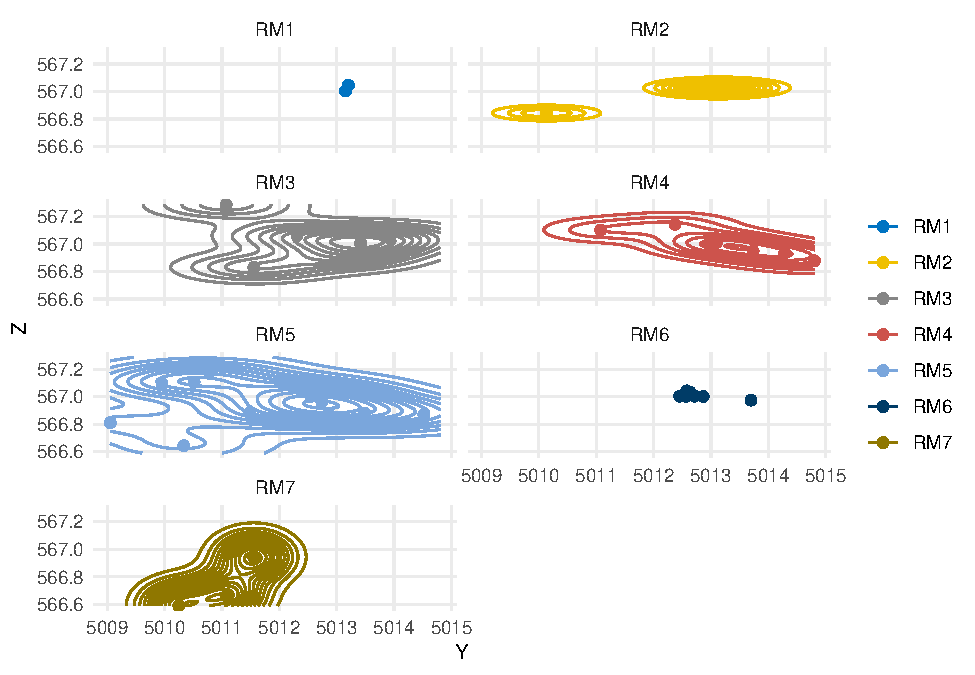
\includegraphics{thesis_files/figure-latex/chertspatial-1.pdf}
\caption{\label{fig:chertspatial}Spatial dispersion (Z vs Y) by chert type using total station data (countors represent a 2D Kernel density estimation).}
\end{figure}
\begin{figure}
\centering
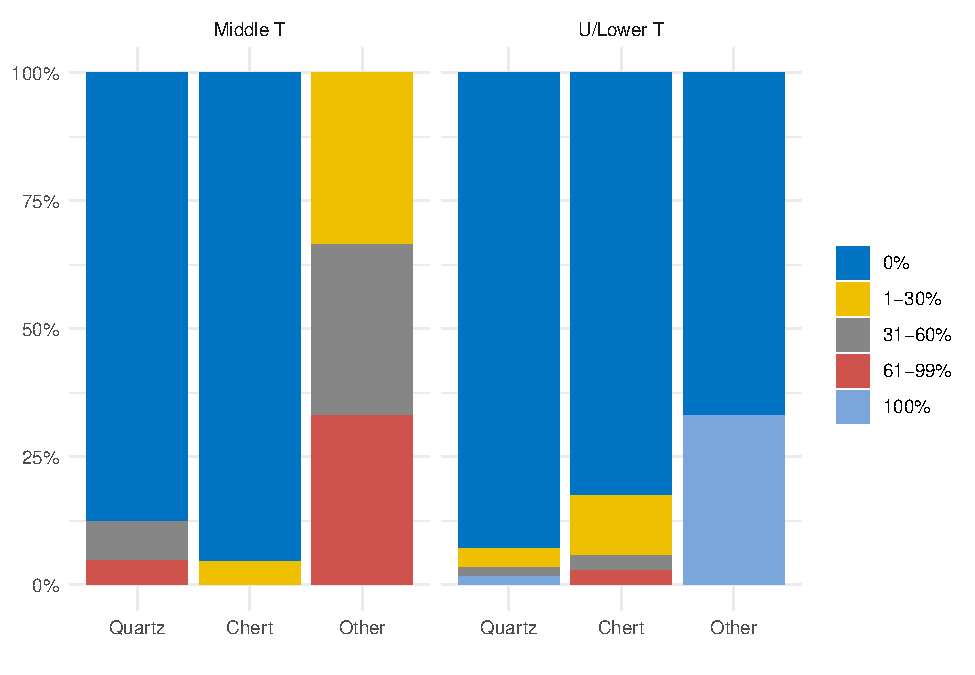
\includegraphics{thesis_files/figure-latex/cortexlp-1.pdf}
\caption{\label{fig:cortexlp}Lapa do Picareiro. Frequencies of cortex by raw material and by phase. Chips and shatters not included}
\end{figure}
\begin{table}

\caption{\label{tab:cortexabtg}Lapa do Picareiro - U/Lower T. Frequencies of cortex type by raw material.}
\centering
\resizebox{\linewidth}{!}{
\begin{tabular}[t]{>{\bfseries}llll}
\toprule
Cortex attributes & Quartz & Chert & Total\\
\midrule
CortexType, n (\%) &  &  & \\
Cobble & 3 (75.0) & 0 (0.0) & 5 (41.7)\\
Indeterminate & 1 (25.0) & 4 (66.7) & 5 (41.7)\\
Outcrop & 0 (0.0) & 2 (33.3) & 2 (16.7)\\
\bottomrule
\end{tabular}}
\end{table}
\begin{table}

\caption{\label{tab:cortextabpr}Lapa do Picareiro - Middle T. Frequencies of cortex type by raw material.}
\centering
\resizebox{\linewidth}{!}{
\begin{tabular}[t]{>{\bfseries}lllll}
\toprule
Cortex attributes & Quartz & Chert & Other & Total\\
\midrule
CortexType, n (\%) &  &  &  & \\
Cobble & 5 (100.0) & 0 (0.0) & 2 (66.7) & 7 (63.6)\\
Indeterminate & 0 (0.0) & 3 (100.0) & 1 (33.3) & 4 (36.4)\\
\bottomrule
\end{tabular}}
\end{table}
\hypertarget{technological-analysis}{%
\section{Technological analysis}\label{technological-analysis}}

\hypertarget{cores}{%
\subsection{Cores}\label{cores}}

\hypertarget{vale-boi-4}{%
\subsubsection{Vale Boi}\label{vale-boi-4}}

The core assemblage from Vale Boi totals 123 pieces, with 46 total pieces coming from the Lower 5 levels, and 77 from the Upper 5/4E group (tables \ref{tab:general1} and \ref{tab:general2}).

Excluding inform cores, which were not considered here because they do not possess all the recordable attributes, there is a clear dominance of single platform cores, for most raw materials and in both phases. Chert presents the highest variability of core types, with high frequencies for single platform (50\% for Lower 5 and 33.3\% in Upper 5/4E), but also prismatic (37.5\% on Lower 5). On Upper 5/4E, there are also opposed, pyramidal, two single platforms and other types of platforms in percentages higher than 10\%. In the Lower 5 group chert unidirectional prismatic cores are more frequent (Figure \ref{fig:coretypeVB}.

This variability can be seen in figures \ref{fig:corelower} and \ref{fig:coreupper}, where vectorized scar cores from Upper 5/4E show a wider variety of scar directionalities and higher scar counts. Comparatively, vectorized cores from Lower 5 all show unidirectional patterns, with a general smaller scar count, thus showing somewhat more homogeneous results.
\begin{figure}

{\centering 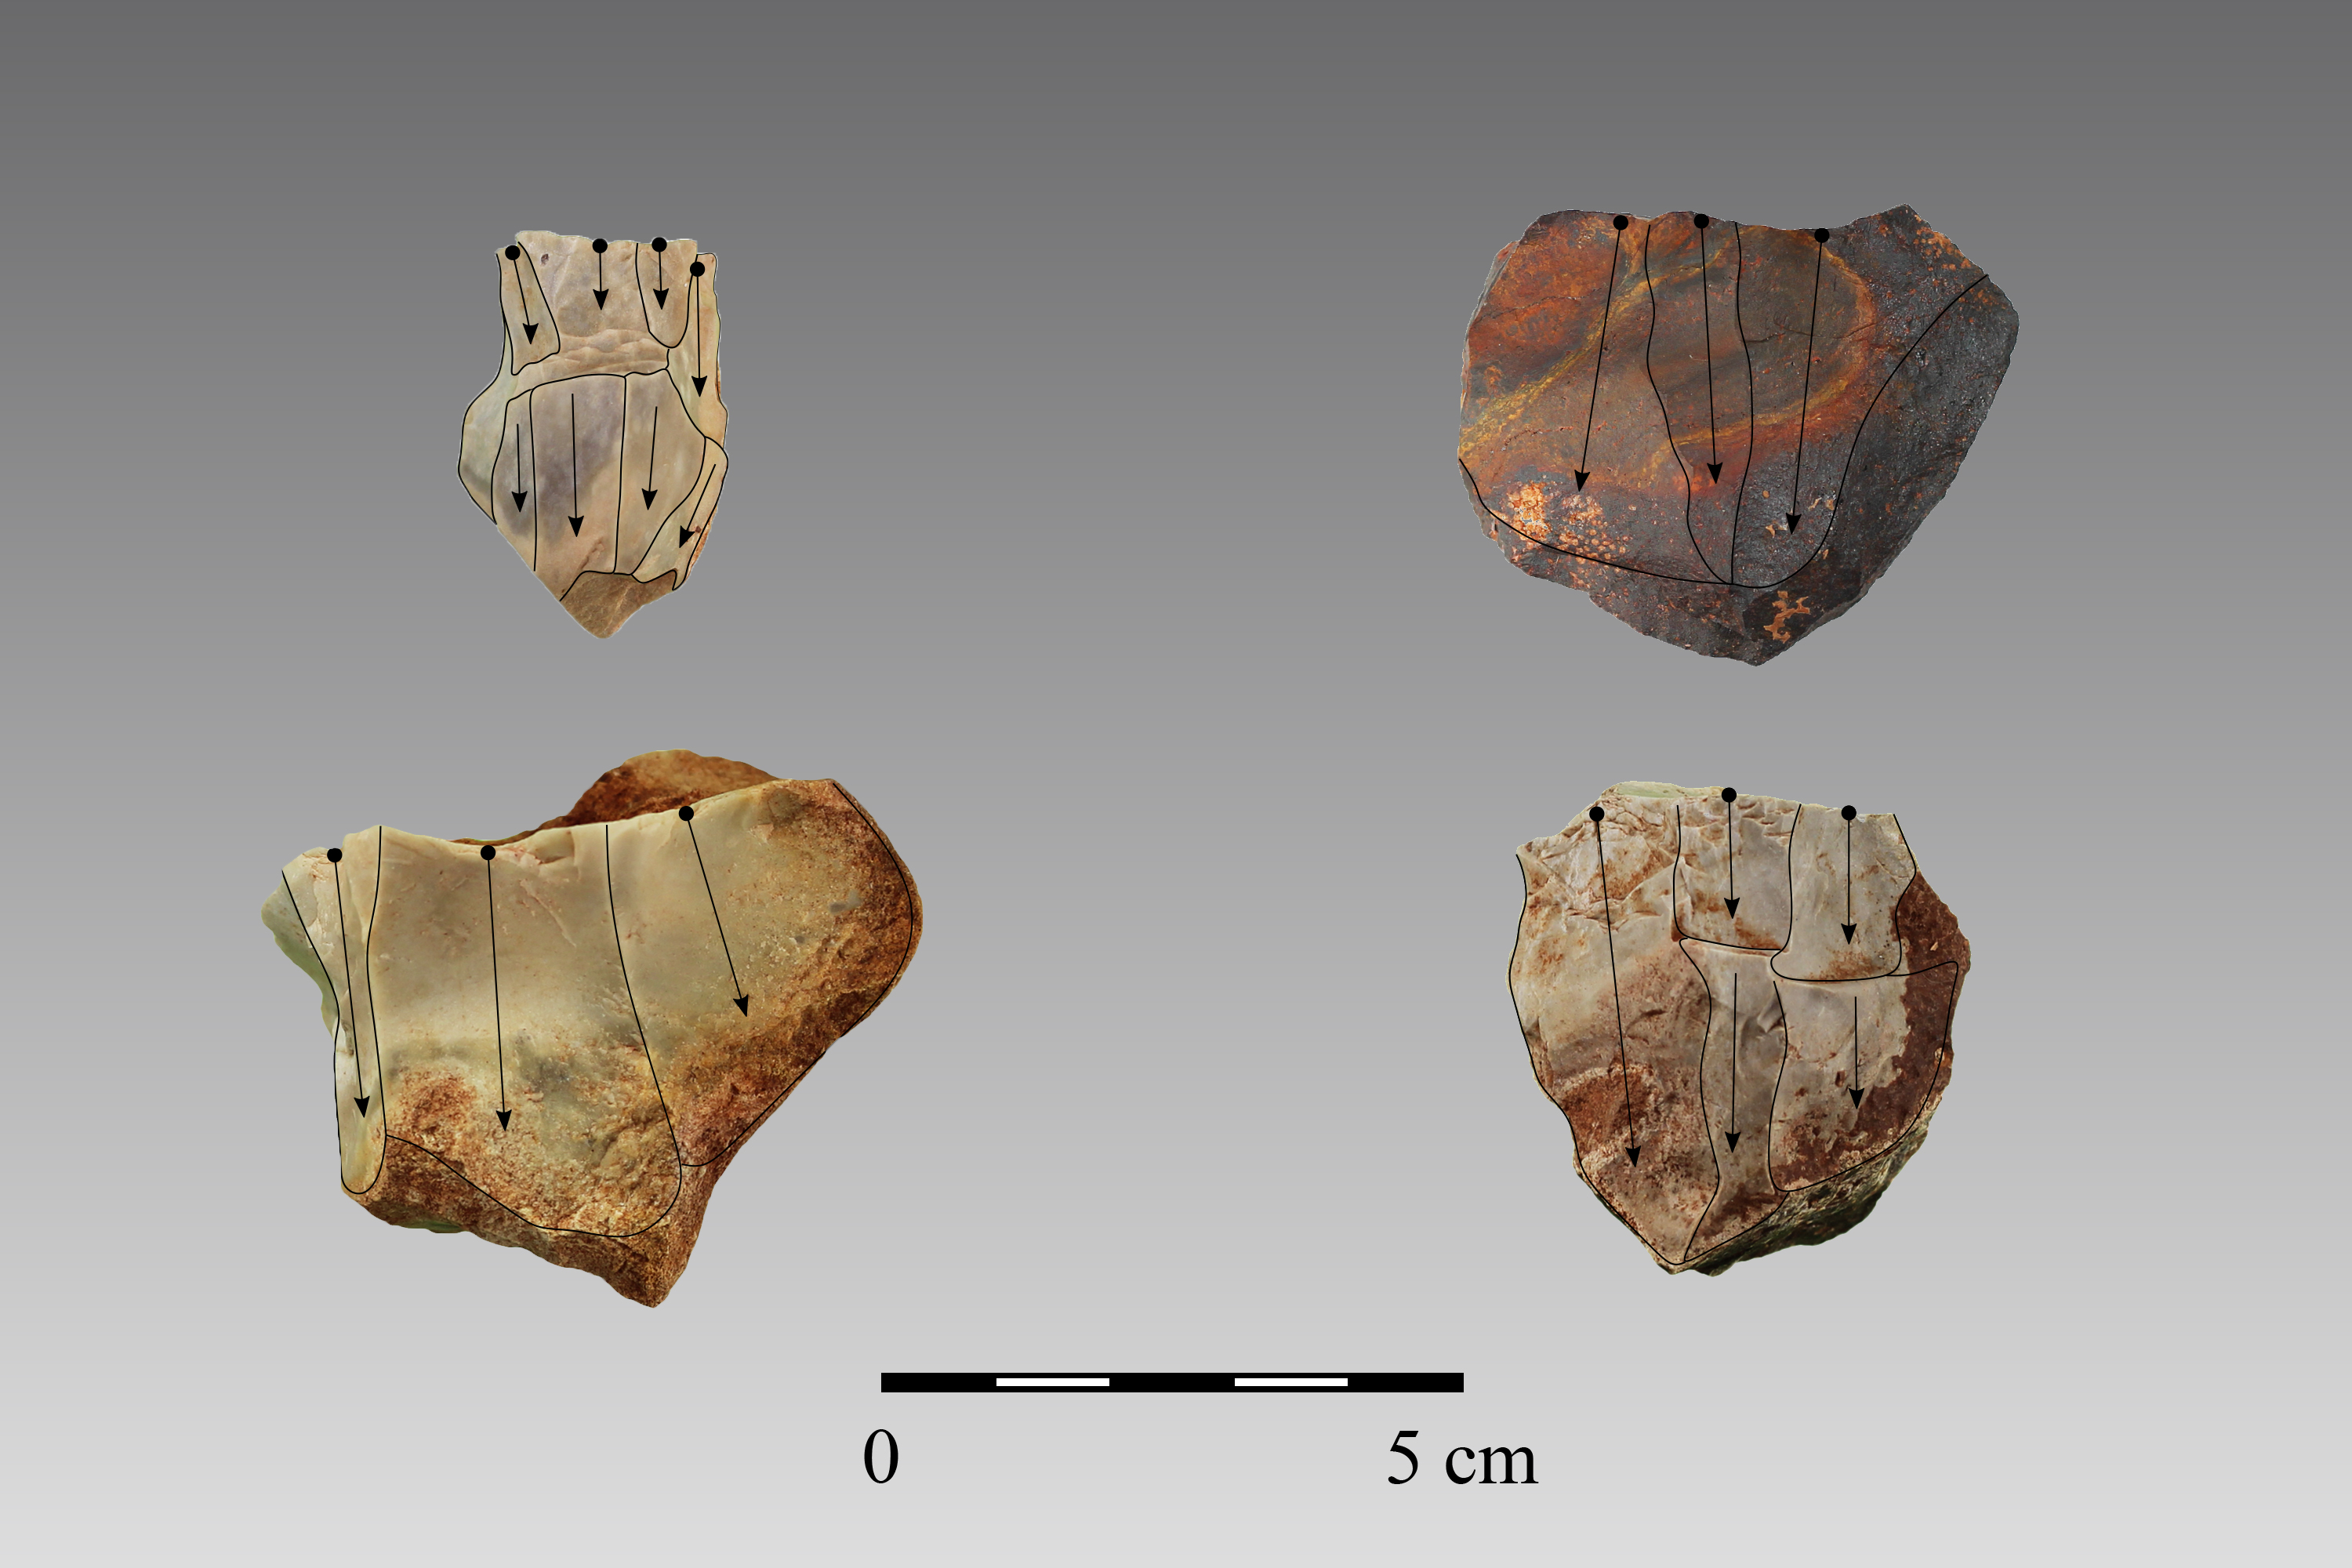
\includegraphics[width=0.8\linewidth]{figure/coreL} 

}

\caption{Vale Boi - Lower 5 - Chert and iron oxide (upper right) cores with vectorized scar negatives and scar directionality.}\label{fig:corelower}
\end{figure}
\begin{figure}

{\centering 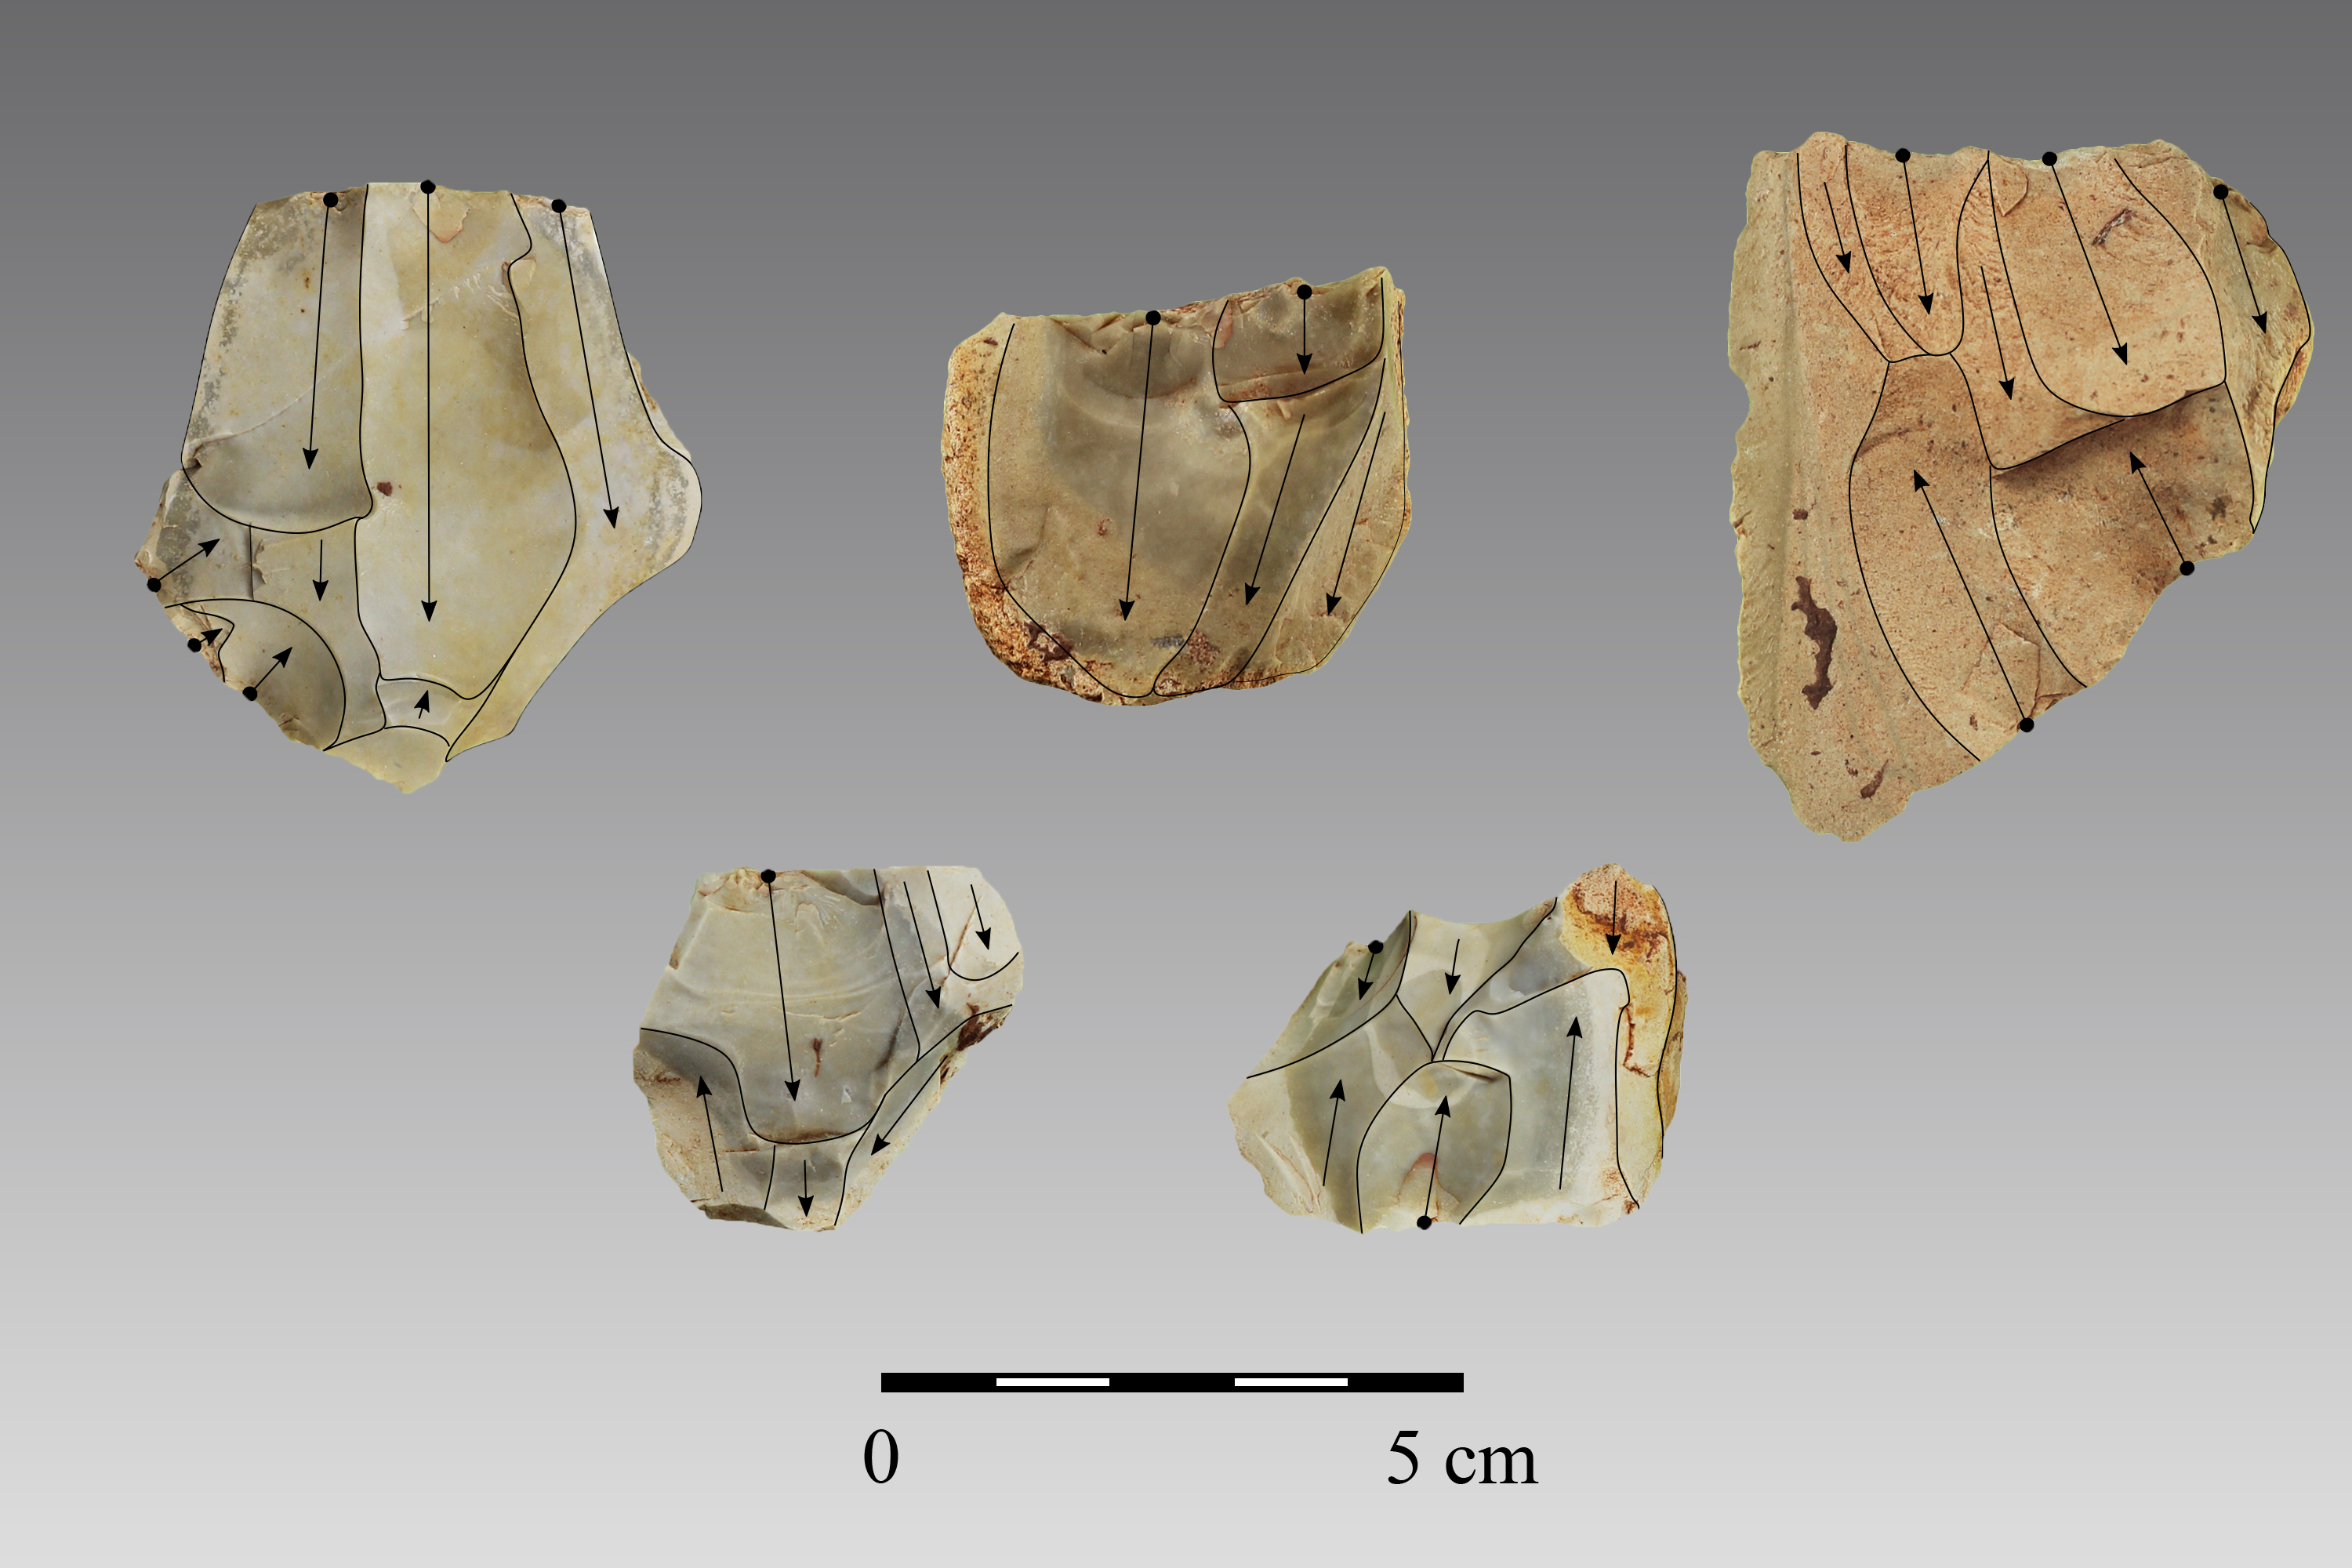
\includegraphics[width=0.8\linewidth]{figure/coreU} 

}

\caption{Vale Boi - Upper 5/4E - Chert cores with vectorized scar negatives and scar directionality.}\label{fig:coreupper}
\end{figure}
Most of the cores were used for the extraction of flakes, although blade and bladelet scars also show relatively high frequencies associated with the exploitation of unidirectional prismatic cores in Lower 5 and Upper5/4E groups (Figure \ref{fig:coretypeVB}).
\begin{figure}
\centering
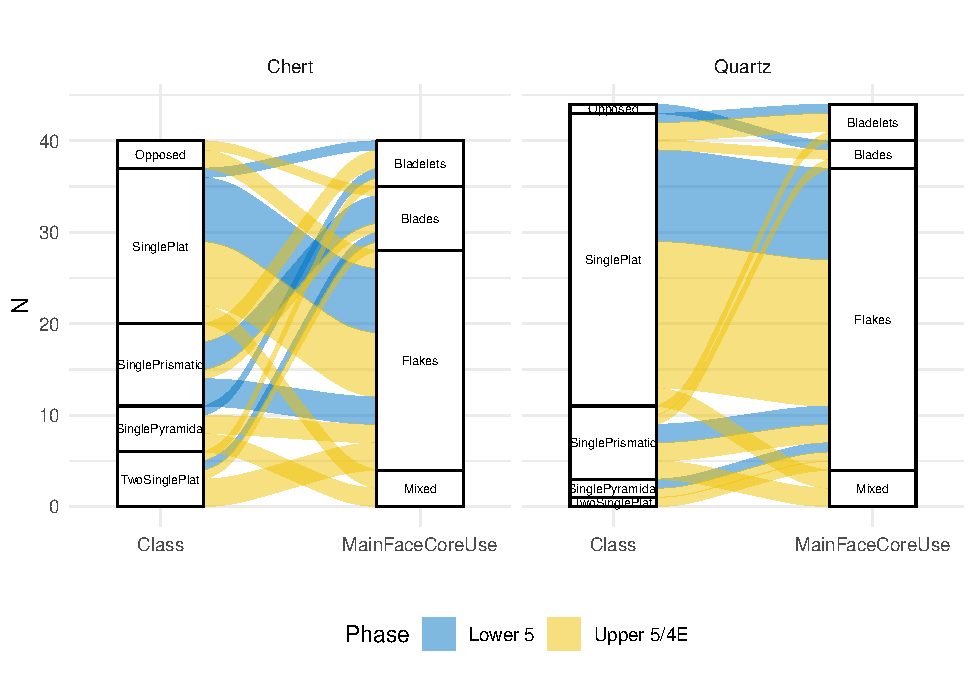
\includegraphics{thesis_files/figure-latex/coretypeVB-1.pdf}
\caption{\label{fig:coretypeVB}Vale Boi. Interaction of core type with type of extracted products by raw material and phase.}
\end{figure}
Most of the analyzed core platforms are plain or cortical. On Upper 5/4E there is a small frequency of faceted platforms on both quartz and chert (3.4\% and 18.5\% respectively). Platforms width and thickness means show smaller platforms for chert on both phases, while greywacke shows the highest means for platform measurements (table \ref{tab:coremetricsVB1} and \ref{tab:coremetricsVB2}). This pattern is similar for other measurements, for which chert and quartz exhibit the smaller means.

Regarding elongation, Figure \ref{tab:coreboxplotVB} shows wider range and higher elongation values for chert cores in both phases. Upper 5/4E seems to have less elongated cores in both chert and quartz, but the t-test results indicate no significant difference between the sets (Chert p-value = 0.498451, Quartz p-value = 0.3166799. Other raw materials, including greywacke, show the lower values for elongation.

Core flattening (Figure \ref{fig:coreboxplotVB}) (calculated by dividing maximum width by thickness) reveals that greywacke and other raw materials show higher values, while quartz and chert cores have similar values for both phases (Chert t-test p-value = 0.847313, Quartz t-test p-value = 0.2651861), with flattening median values of around 1.5, centered in between the second and third quartiles of the distribution.
\begin{figure}
\centering
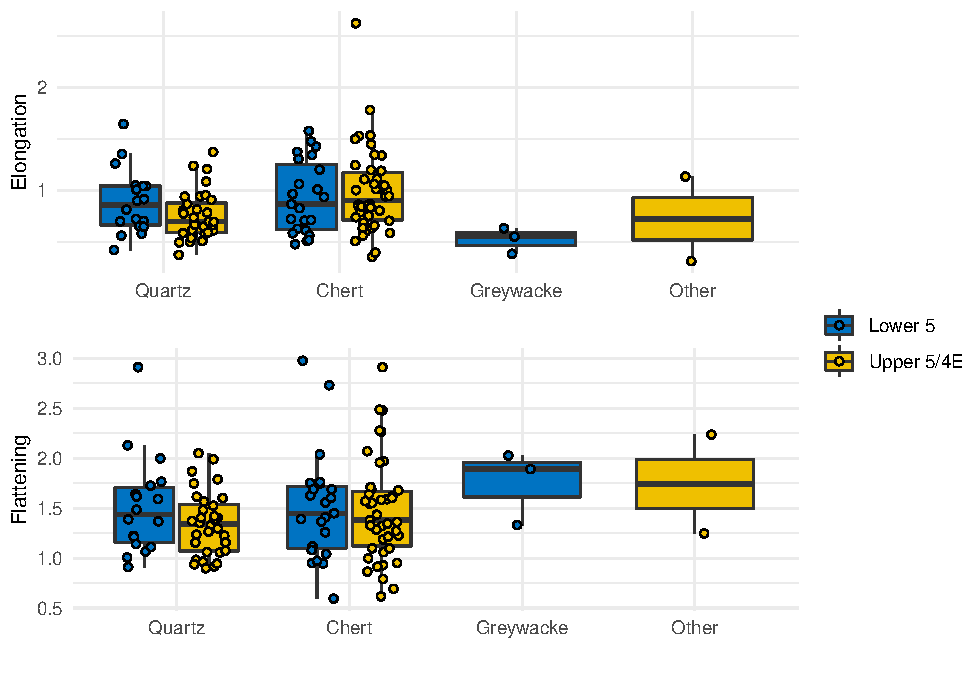
\includegraphics{thesis_files/figure-latex/corebloxplotVB-1.pdf}
\caption{\label{fig:corebloxplotVB}Vale Boi. Boxplots of core elongation and flattening by raw material and phase.}
\end{figure}
\hypertarget{lapa-do-picareiro-4}{%
\subsubsection{Lapa do Picareiro}\label{lapa-do-picareiro-4}}

A total of seven cores were recorded on the Lapa do Picareiro assemblages, two in the U/Lower T group (both in quartz) and five in the Middle T, of which two are in chert and two are in quartz.

Single platform, prismatic and pyramidal cores were identified in the Middle T group (table \ref{tab:coreattributesLP2}. These were mainly used to remove flakes (Figure \ref{fig:coretypeLP}) and only prismatic cores showed evidence for the production of mixed blanks. Platforms tend to be unfacetted, although a small number of cores presented dihedral platforms (2 in Middle T, in quartz and chert). The number of debitage surfaces is greater on chert cores for the Middle T group, while quartz varies between single and three faces (tables \ref{tab:coreattributesLP1} and \ref{tab:coreattributesLP2}).

Metrically, chert has smaller mean values for all core measurements when compared to other raw materials (tables \ref{tab:coremetricsLP1} and \ref{tab:coremetricsLP2}), showing, however, higher elongation ratios (Figure \ref{fig:coreboxplotLP}). Regarding quartz cores, the differences between the U/Lower T phase and the Middle T phase are very obvious, with the first group showing more elongated cores with low flattening values. However, these differences may simply be the result of the rather small number of cores present in the assemblage and a consequent low intra-assemblage variability.
\begin{figure}
\centering
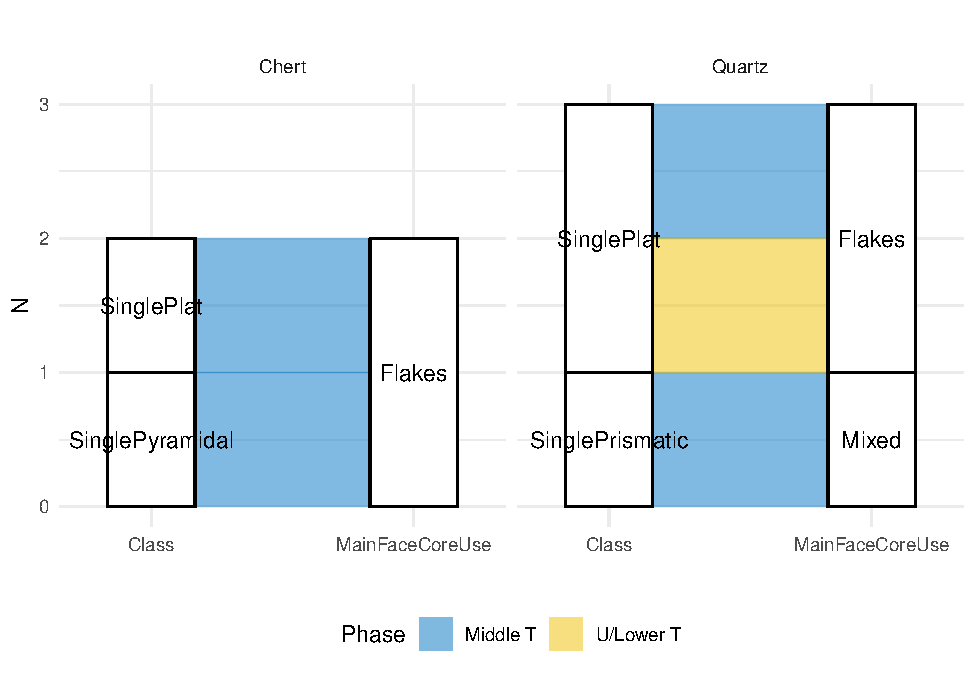
\includegraphics{thesis_files/figure-latex/coretypeLP-1.pdf}
\caption{\label{fig:coretypeLP}Vale Boi. Interaction of core type with type of extracted products by raw material and phase.}
\end{figure}
\begin{figure}
\centering
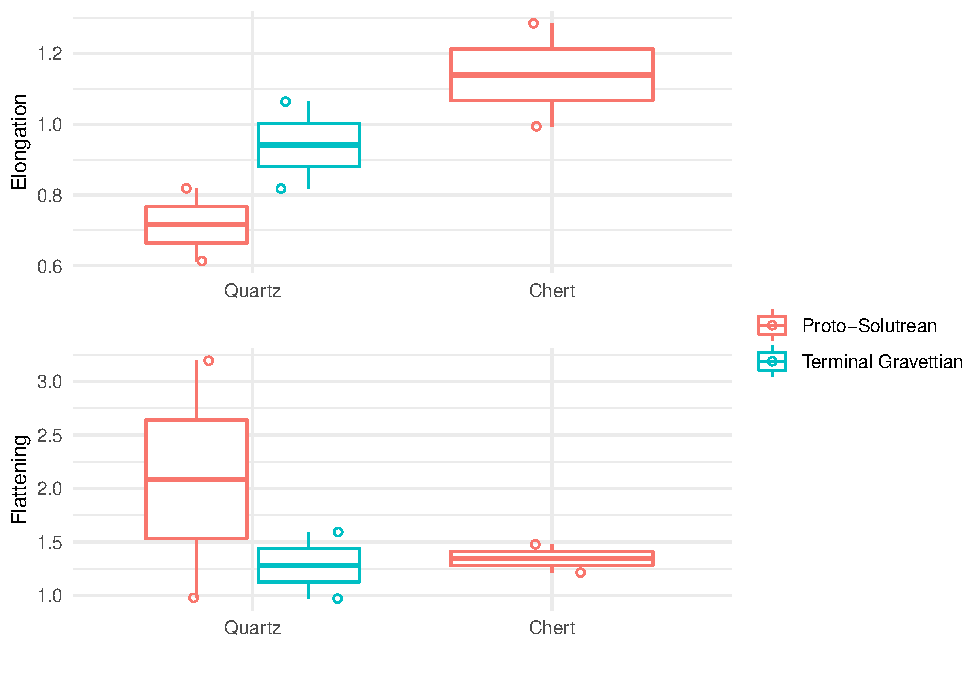
\includegraphics{thesis_files/figure-latex/corebloxplotLP-1.pdf}
\caption{\label{fig:corebloxplotLP}Lapa do Picareiro. Boxplots of core elongation and flattening by raw material and phase.}
\end{figure}
\hypertarget{core-maintenance-products}{%
\subsection{Core maintenance products}\label{core-maintenance-products}}

Core maintenance products are very scarce in the assemblages from both sites, with a single identified piece at Lapa do Picareiro's U/Lower T phase (a chert core tablet), and a total of seven pieces for Vale Boi's assemblages, of which six artifacts come from the Upper 5/4E levels.

At Vale Boi core maintenance products are of two types, core fronts and core tablets (Table \ref{tab:corepreptypeVB}). Most core maintenance products are on chert (n=5) with only two quartz core tablets identified, one for each phase.

No cortex was present in the dorsal surfaces of all core maintenance products. This pattern reveals that maintenance operations were performed at advanced stages of the reduction sequence.

Finnaly, it is rather interesting the absence of crested pieces from both assemblages, mostly at Vale Boi, where this type of core maintenance product has been referenced for both Solutrean and Gravettian occupations (J. M. M. Cascalheira, 2013; Marreiros, 2009).
\begin{table}

\caption{\label{tab:corepreptypeVB}Core maintenance products by raw material for Upper 5/4E.}
\centering
\begin{tabular}[t]{>{\bfseries}lrrr}
\toprule
Core maintenance product & Chert & Quartz & Total\\
\midrule
CoreFront & 3 & 0 & 3\\
CoreTablet & 2 & 1 & 3\\
Total & 5 & 1 & 6\\
\bottomrule
\end{tabular}
\end{table}
\hypertarget{flakes}{%
\subsection{Flakes}\label{flakes}}

\hypertarget{vale-boi-5}{%
\subsubsection{Vale Boi}\label{vale-boi-5}}

A total of 1255 flakes were analysed from Vale Boi, 427 of those belonging to Lower 5 group, and 828 to the Upper 5/4E group. This increase was somehow expected according to the aforementioned general intensity of occupation and material density in the transition from one phase to the other. Although there are generally more flakes in quartz, it is obvious the difference in ratios between chert and quartz, when comparing Lower 5 to Upper 5/4E results.
\begin{figure}
\centering
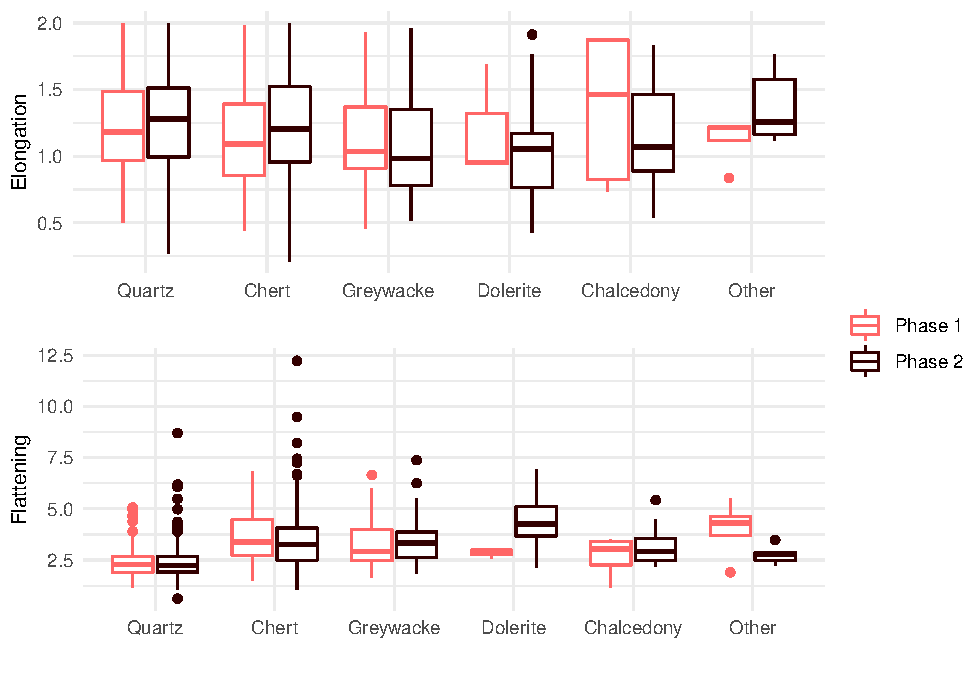
\includegraphics{thesis_files/figure-latex/flakeboxplot-1.pdf}
\caption{\label{fig:flakeboxplot}Vale Boi. Boxplots of flake elongation and flattening by raw material and phase.}
\end{figure}
Morphologically, Lower 5 flakes seem to have mostly irregular shapes, with frequencies over 45\% for most raw materials, followed by convergent and parallel shapes in much lower frequencies (under 15\%) (table \ref{tab:flakeattributeVB1}). Dolerite, unlike other raw materials, shows only convergent and parallel shapes even if with low representativity (n=3). Cross sections are mostly irregular and triangular, varying slightly in frequency regarding each raw material. All raw materials, with exception of quartz, show high frequencies of straight profiles (over 40\%), chert showing a similar percentage between straight and curved profiles (44.3\% and 42.9\% respectively). Quartz, however, has a frequency of 65\% of straight profiles, showing much smaller frequencies for other types.

On Upper 5/4E (table \ref{tab:flakeattributeVB2}), irregular shapes are still frequent, representing over 25\% on all raw materials. Convergent and parallel shapes show higher frequencies (over 20\%) for quartz, chert and dolerite. Alike Lower 5, cross sections are mostly irregular (over 35\% for most raw materials) or triangular (over 25\% for all raw materials), and profile type show the same patterns and similar percentages as Lower 5.

Unidirectional scar patterns are dominant in both phases and all raw materials, with frequencies over 80\%. Bidirectional patterns are slightly more relevant in chert (9.3\%), and also in dolerite and chalcedony during Upper 5/4E. Dorsal patterns also show a dominance on both phases of 1, 2 and 3 scars for most raw materials, although chert shows the widest numbers and variety for higher scar counts.

Flakes have mostly plain platforms, although for certain raw materials, like quartz, there is a relevant presence of crushed platforms (33.3\% for Lower 5 and 35.9\% for Upper 5/4E). Faceted platforms are present in both phases but in low frequencies, in chert for both Lower 5 (1.4\%) and Upper 5/4E (2.4\%), but in no other raw material. Platforms are also mostly non-cortical (between 80\% and 100\% depending on raw material) in both phases.

Blank metrics, including platform measurements, show for Lower 5 (table \ref{tab:flakemetricsVB1}), the smallest means in chalcedony and dolerite, followed by chert and quartz, where greywacke mean values show bigger Flakes in this raw material. On Upper 5/4E (table \ref{tab:flakemetricsVB2}), however, the smallest Flakes are in chert, followed by quartz and chalcedony, where dolerite mean values are fairly closer to those of greywacke, thus making these the Flakes with highest metric mean values.

Regarding elongation (figure \ref{fig:flakeboxplot}), quartz, chert and chalcedony show the highest values, although the latter raw material shows a bigger concentration of similar elongation flakes in the third quartil, thus showing less general elongation (Chert t-test p-value = 0.0157551, Quartz t-test p-value = 0.094501). Despite having similar elongation ranges in both groups, quartz shows relatively different medians, on Lower 5 showing a less variability in the lower quartil, while Upper 5/4E shows lower variability in the upper quartil, hinting at a bigger number of consistently elongated quartz flakes in Upper 5/4E. For chert, Upper 5/4E also seems to show higher elongation values for flakes, though once again, there is a wide range of variability within regarding elongation in the assemblage.

As for flattening (figure \ref{fig:flakeboxplot}), quartz shows very low values for flake flattening, compared to other raw materials (Chert t-test p-value = 0.9364755, Quartz t-test p-value = 0.6089536). The data, however, also shows the existance of a wide variability within each raw material, with the existance of several outliers which fall from the statistical groupings and quartils. As such, it seems that for all raw materials, perhaps with the exception of quartz, flake flattening is extremely variable in the assemblage.

\hypertarget{lapa-do-picareiro-5}{%
\subsubsection{Lapa do Picareiro}\label{lapa-do-picareiro-5}}

There are a total of plotted 122 Flakes, 46 attributed to the U/Lower T group, more than 50\% being in quartz, and 67 attributed to the Middle T group, its vast majority in chert. On both groups, attributes are very similar.

On the U/Lower T phase, for quartz, there seems to be the predominance of parallel shapes (35\%) (table \ref{tab:flakeattributesLP1}), followed by convergent ones (30\%). Chert, however, shows higher percentages for irregular (28.6\%) and divergent (42.9\%) shapes. Cross sections are mostly triangular for all raw materials (over 40\%), although chert also shows high frequencies of trapezoidal cross sections (42.9\%). Profiles are, for all raw materials, mostly straight (60\% on quartz and 85.7\% on chert) and terminations show relevant raw material differences, with quartz having bigger frequencies of feathered and hinged terminations (35\% and 40\% respectively) and chert having a frequency of 42.9\% on pointed terminations. For all raw materials, there is the predominance of unidirectional dorsal patterns, high frequencies over 85\%. Dorsal scars show higher frequencies for 2 and 3 scars on quartz (35\% and 40\% respectively), while other raw materials show higher frequencies for 3 dorsal scars only (42.9\% on chert).

On the Middle T phase (table \ref{tab:flakeattributesLP2}), quartz shows higher frequencies for irregular shapes (53.8\%), followed by convergent ones (38.5\%). Contrary to the patterns seen on the previous group, chert shows higher frequencies for parallel shapes (40.6\%). For all raw materials, cross sections are predominantly triangular (over 40\%) with straight profiles (over 50\%) and feathered terminations for chert (40.6\%), whereas quartz shows higher values for hinged terminations (46.2\%) followed by feathered (38.5\%). Alike the U/Lower T group, there is the predominance of unidirectional dorsal scar patterns (over 90\% for all raw materials), with high frequencies for 2 dorsal scars in quartz (61.5\%) and 2-3 dorsal scars in chert (34.4\% both).

Regarding platforms, for both groups, they are mostly plain for all raw materials (over 40\%), followed by relatively high values of crushed platforms in quartz, with the presence of 1 faceted platform for quartz and chert in each group. Chert on the Middle T group also shows dihedral platforms (18.8\%). Platforms seem to have barely any cortex, for all raw materials in both groups.

Measurements, including platform width and thickness, show larger means for the chert flakes (19.5 mm width and 27.3 mm length), comparatively to the quartz ones (16.7 mm width and 21.8 mm length), for Lower 5 (table \ref{tab:flakemetricsLP1}) and for Upper 5/4E (table \ref{tab:flakemetricsLP2})(chert with 17.2 mm width and 20.9 mm length, and quartz with 13 mm width and 16.3 mm length). There also seems to be a size difference between groups, with the U/Lower T flakes showing bigger means (although with high standard deviation values), while Middle T means show smaller values and smaller SD values, the only constant seeming to be the thickness of flakes on chert (5-5.3 mm), wich seem to show little variability (standard deviations of 3.1 for the U/Lower T group and 2.3 for the Middle T group).
\begin{figure}
\centering
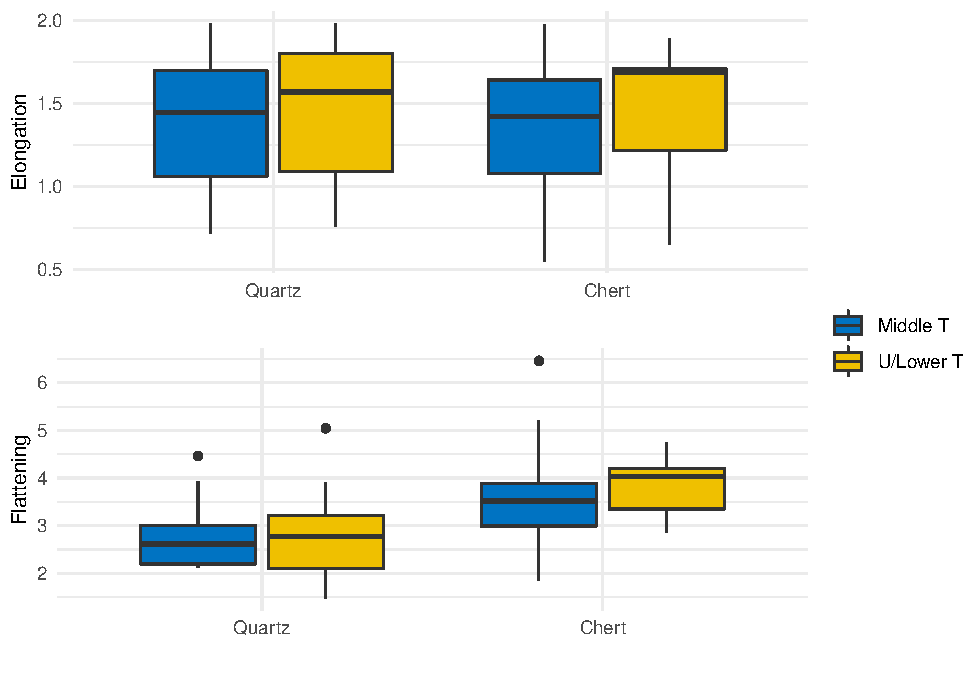
\includegraphics{thesis_files/figure-latex/flakeboxplotLP-1.pdf}
\caption{\label{fig:flakeboxplotLP}Flake elongation and flattening by phase and raw material.}
\end{figure}
Regarding elongation (figure X), values between quartz and chert and even between groups seem to be fairly similar, all with elongation ratios which seem skewed above, thus showing less elongation variability above the 1.5 threshold (Chert t-test p-value = 0.5558095, Quartz t-test p-value = 0.9095166).

Flake flattening, however, shows more apparent differences between raw materials, with quartz showing lower flattening ratios than chert (Chert t-test p-value = 0.4703381, Quartz t-test p-value = 0.8611236). Within chert, however, there also seems to be a difference in general flattening variability and interquartil skewness, showing a larger number of flakes with similar flattening values (at around 4).

\hypertarget{elongated-blanks}{%
\subsection{Elongated blanks}\label{elongated-blanks}}

\hypertarget{vale-boi-6}{%
\subsubsection{Vale Boi}\label{vale-boi-6}}

A total of 219 elongated products were recorded in the Vale Boi's assemblages. 82 of these blanks are from Lower 5, while 137 are from the Upper 5/4E group. Comparatively to the whole group of blanks, there is a more significant number of chert pieces (n=106), this number only changing in Lower 5, where quartz elongated blank numbers (n=44) supersede chert ones (n=31). Figures \ref{fig:elongdisp1} and \ref{fig:elongdisp2} show the scatterplots for width and length of elongated blanks of the two main raw materials present at both phases identified at Vale Boi. Following the traditional subdivision between blade and bladelet, both charts clearly show that the main goal of the reduction sequences for elongated products were bladelets. Only in the Upper 5/4E group, there seems to be a bimodal distribution in the width variable for chert artifacts.

Testing this apparent division (artifacts wider than 12.5 mm and those with less than 12.5 in width) against all other relevant morphological variables revealed, however, no significant difference between the two groups for almost all variables (Table \ref{tab:fisherelongVB2}). The exception to this pattern were the tests for scar count, scar pattern and cortex presence. In the first case, due to a more substantial presence of three scars on the blade products and two scars on the bladelet products. In the second case because of the higher frequency (c.~13\% vs.~c.~2\%) of bidirectional removals on the dorsal surfaces of blades and bladelets, respectively. Finally, in the third case, as a result of the higher frequencies of cortical surfaces recorded for blades (c.~67\%) vs.~bladelets (c.~18\%). Altogether, these results seem to indicate that the difference between the two classes is likely not related with the existence of two distinct reduction sequences but of a single reduction sequence with cortical or partially cortical elongated products at the beginning of core exploitation, when bidirectional strategies were used to perform decortication and core configuration. Together with the reasonably linear positive correlation showed by the chert tendency line displayed in Figure \ref{fig:elongdisp2}, the results seem enough to do the technological description of all elongated products as a single category.
\begin{figure}
\centering
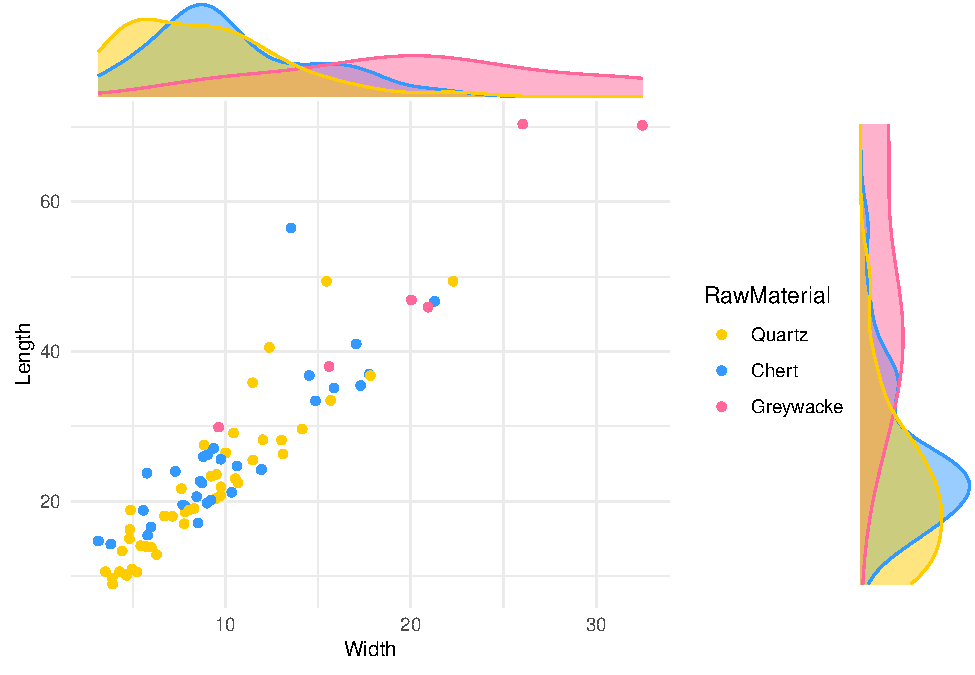
\includegraphics{thesis_files/figure-latex/elongdisp1-1.pdf}
\caption{\label{fig:elongdisp1}Vale Boi - Lower 5. Elongated products width and length dispersion by raw material.}
\end{figure}
\begin{figure}
\centering
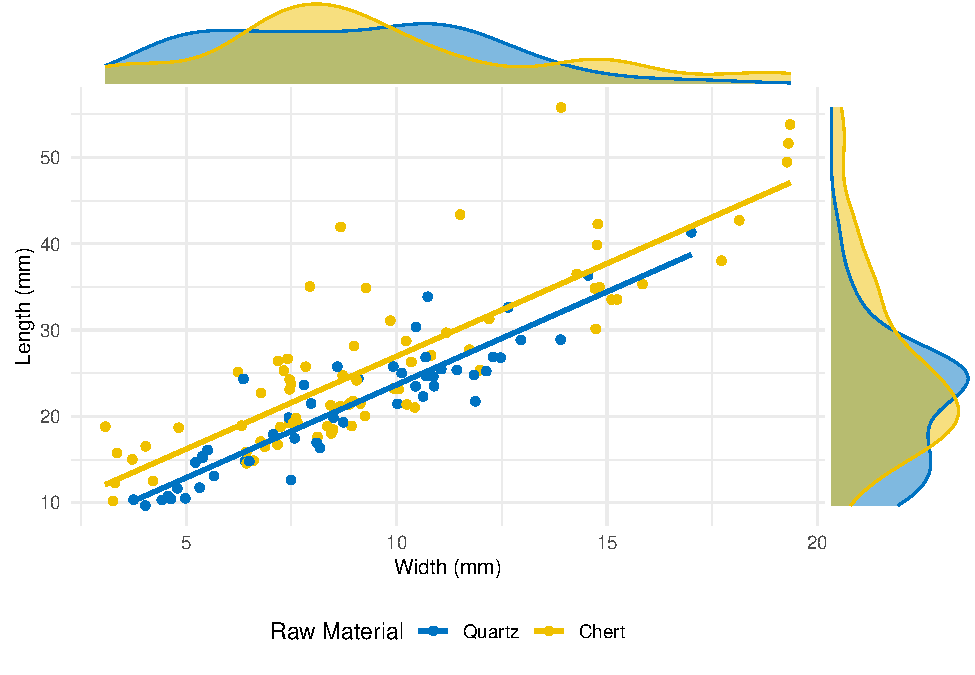
\includegraphics{thesis_files/figure-latex/elongdisp2-1.pdf}
\caption{\label{fig:elongdisp2}Vale Boi - Upper 5/4E. Elongated product width and length dispersion by raw material.}
\end{figure}
\begin{longtable}[t]{llll}
\caption{\label{tab:fisherelongVB2}Vale Boi - Upper5/4E. Results of Fisher exact tests to evaluate whether the distribution of technological variables differed across metric groups (blades and bladelets) of chert elongated artifacts.}\\
\toprule
\multicolumn{1}{c}{\textbf{Attributes}} & \multicolumn{1}{c}{\textbf{Blade}} & \multicolumn{1}{c}{\textbf{Bladelet}} & \multicolumn{1}{c}{\textbf{P}}\\
\midrule
CrossSection, n (\%) &  &  & 0.24\\
Irregular & 3 (20.0) & 3 (5.0) & \\
Lenticular & 0 (0.0) & 3 (5.0) & \\
Quadrangular & 0 (0.0) & 2 (3.3) & \\
Trapezoidal & 3 (20.0) & 7 (11.7) & \\
\addlinespace
Triangular & 9 (60.0) & 45 (75.0) & \\
BlankShape, n (\%) &  &  & 0.54\\
Convergent & 6 (40.0) & 22 (36.7) & \\
Divergent & 0 (0.0) & 6 (10.0) & \\
Irregular & 1 (6.7) & 9 (15.0) & \\
\addlinespace
Parallel & 8 (53.3) & 23 (38.3) & \\
Profile, n (\%) &  &  & 0.22\\
Curved & 8 (53.3) & 18 (30.0) & \\
Irregular & 1 (6.7) & 4 (6.7) & \\
Straight & 6 (40.0) & 29 (48.3) & \\
\addlinespace
Twisted & 0 (0.0) & 9 (15.0) & \\
BlankTip, n (\%) &  &  & 0.52\\
Feather & 4 (26.7) & 23 (38.3) & \\
Hinge & 3 (20.0) & 14 (23.3) & \\
Overshoot & 1 (6.7) & 3 (5.0) & \\
\addlinespace
Pointed & 3 (20.0) & 14 (23.3) & \\
Step & 4 (26.7) & 6 (10.0) & \\
PlatformType, n (\%) &  &  & 0.53\\
Crushed & 1 (6.7) & 10 (16.7) & \\
Dihedral & 0 (0.0) & 3 (5.0) & \\
\addlinespace
Faceted & 0 (0.0) & 1 (1.7) & \\
Linear & 0 (0.0) & 7 (11.7) & \\
Plain & 14 (93.3) & 38 (63.3) & \\
Winged & 0 (0.0) & 1 (1.7) & \\
PlatformCortex, n (\%) &  &  & 0.11\\
\addlinespace
No & 11 (73.3) & 54 (90.0) & \\
YesComplete & 4 (26.7) & 6 (10.0) & \\
Cortex, n (\%) &  &  & 0.001\\
0\% & 5 (33.3) & 49 (81.7) & \\
1-30\% & 5 (33.3) & 5 (8.3) & \\
\addlinespace
100\% & 1 (6.7) & 0 (0.0) & \\
31-60\% & 3 (20.0) & 3 (5.0) & \\
61-99\% & 1 (6.7) & 3 (5.0) & \\
ScarCount, n (\%) &  &  & 0.005\\
0 & 1 (6.7) & 0 (0.0) & \\
\addlinespace
1 & 3 (20.0) & 2 (3.3) & \\
2 & 2 (13.3) & 32 (53.3) & \\
3 & 9 (60.0) & 23 (38.3) & \\
4 & 0 (0.0) & 2 (3.3) & \\
5 & 0 (0.0) & 1 (1.7) & \\
\addlinespace
ScarPattern, n (\%) &  &  & 0.02\\
Bidirectional & 2 (13.3) & 1 (1.7) & \\
None & 1 (6.7) & 0 (0.0) & \\
Unidirectional & 12 (80.0) & 59 (98.3) & \\
\bottomrule
\end{longtable}
Regarding morphology, elongated blanks have mostly parallel and convergent shapes, on both phases, although Lower 5 shows significant differences across the different raw materials, since c.~64\% of quartz has parallel shapes, whereas c.~52\% of chert has convergent ones. Cross sections are mostly triangular, with straight and curved profiles. Differences in profile types are rather significant between both phases, but only for quartz artifacts. While in Lower 5, quartz elongated blanks present a percentage of curved profiles of c.~23\%, in Upper 5/4E, this percentage drops to c.~12\%. Curved and twisted profiles in bladelets are usually associated with the exploitation of carinated cores, particularly in the Gravettian-Solutrean transition as presented by Almeida (2000) for the Terminal Gravettian of Estremadura. Although no carinated cores were identified in the Lower 5 assemblage, the presence of a significant number of bladelets with curved profiles might indicate the use of such a type of reduction strategy.

Scar patterns show an evident tendency for unidirectional knapping strategies on all raw materials. For Lower 5, however, bidirectional scar patterns are present on two chert artifacts (c.~13\%). Upper 5/4E shows much lower values for this type of scar pattern, with c.~2\% on quartz and c.~4\% on chert. Scar count shows a tendency for 1 to 3 dorsal scars on both phases and all raw materials.

Elongated blanks on both phases seem to be obtained without platform preparation, although quartz also shows a significant presence of crushed platforms. Only two faceted platforms were identified, in Upper 5/4E, on chert and dolerite pieces. The general tendency for both phases is for the absence of cortical platforms. Only chert and greywacke on Lower 5 (c.~10\% and c.~17\% respectively) and chert on Upper 5/4E (c.~13\%) show completely cortical platforms.

Finally, elongated products metrics, including platform measurements, show a tendency on both phases for smaller blanks on quartz, followed by chert, whereas greywacke, dolerite and chalcedony show the biggest blanks and widest platforms. On both phases, means for width, length and thickness for quartz and chert are around 9mm, 21-26mm, and 5mm, respectively. Higher standard deviation values are observed for length. Despite this, chert elongated blanks seem to show means which hint for higher elongation ratios than quartz.

\hypertarget{lapa-do-picareiro-6}{%
\subsubsection{Lapa do Picareiro}\label{lapa-do-picareiro-6}}

A total of 47 elongated blanks were recorded for Lapa do Picareiro. U/Lower T phase contains 27 in total, of which more than 50\% are on chert. For the Middle T phase, 20 elongated blanks were recorded, with also more than 50\% on chert.

When plotting width and length for elongated blanks, for chert and quartz, there seem to be two groups of different dimensions in both phases. Concerning the U/Lower T (fig.~\ref{fig:elongdisp1LP}), there is a group of smaller blanks, ranging between 2-10 mm of width and 5-25 mm of length, thus falling into the traditional category of bladelet, and a group that although more disperse is composed mostly of chert, with width and length ranging between 13-26 mm and 40-60 mm, respectively, and that may be classified, according to the traditional definition, as blades.

For the Middle T (fig.~\ref{fig:elongdisp2LP}), there is also a group of smaller blanks, with widths ranging from 3 to 10mm, and highly variable length values, ranging from between 5 to 30mm, from which the higher values represent mostly chert artifacts. Even so, these pieces may be characterized through the traditional classification as bladelets. The second group is made up entirely of chert, although it has fewer blanks and is very disperse in terms of width (\textgreater15mm), and length (\textgreater45mm), and thus classified as blades.

These patterns may represent different production strategies for specific chert elongated blank sizes, although, given the location of the site, it might merely reflect the truncated nature of the reduction sequences present at the site, only showing the presence of two groups of bladelets and blades.

Tables \ref{tab:fisherelongLP1} and \ref{tab:fisherelongLP2} show the results of Fisher exact tests to evaluate whether the distribution of all the relevant technological variables differed across groups of chert artifacts. No significant statistical differences were detected in any of the technological variables for both phases.

In fact, both blades and bladelets show a majority of parallel and convergent edge shapes, straight and curved profiles. Dorsal scars are unidirectional on the dorsal surfaces of all artifacts, with a majority of two previous removals for quartz and two to four scars for chert. Platforms are mostly plain, with no cortex (table \ref{tab:elongtableLP1} and \ref{tab:elongtableLP2}).
\begin{figure}
\centering
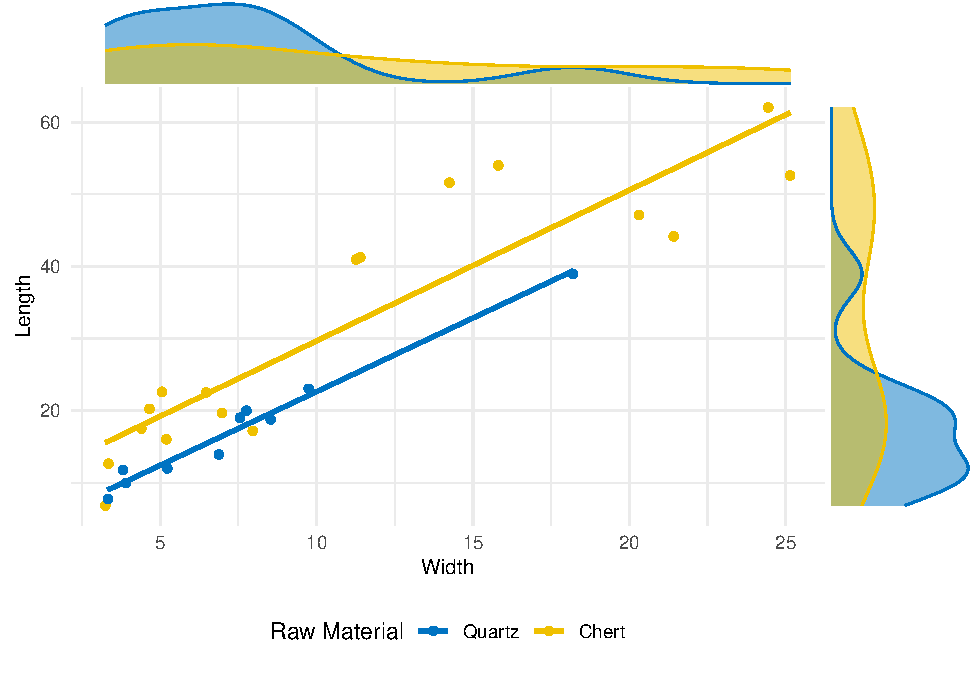
\includegraphics{thesis_files/figure-latex/elongdisp1LP-1.pdf}
\caption{\label{fig:elongdisp1LP}Lapa do Picareiro - U/Lower T. Elongated product width and length dispersion by raw material.}
\end{figure}
\begin{figure}
\centering
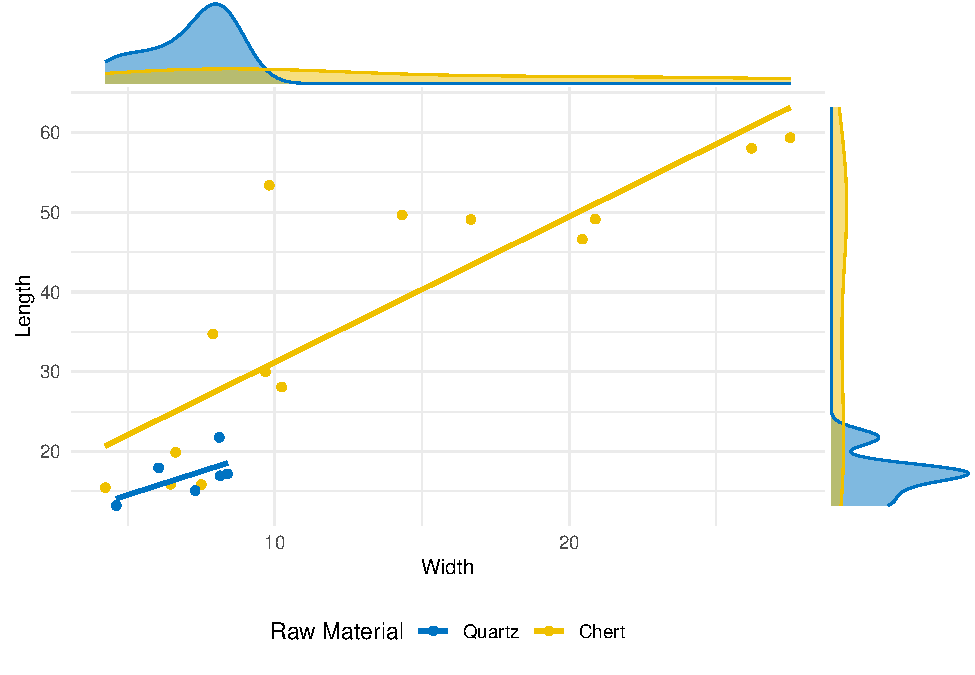
\includegraphics{thesis_files/figure-latex/elongdisp2LP-1.pdf}
\caption{\label{fig:elongdisp2LP}Lapa do Picareiro - Middle T. Elongated product width and length dispersion by raw material.}
\end{figure}
\begin{longtable}[t]{llll}
\caption{\label{tab:fisherelongLP1}Lapa do Picareiro - U/Lower T. Results of Fisher exact tests to evaluate whether the distribution of technological variables differed across metric groups (blades and bladelets) of chert elongated artifacts.}\\
\toprule
\multicolumn{1}{c}{\textbf{Attributes}} & \multicolumn{1}{c}{\textbf{Blade}} & \multicolumn{1}{c}{\textbf{Bladelet}} & \multicolumn{1}{c}{\textbf{P}}\\
\midrule
CrossSection, n (\%) &  &  & 0.73\\
Irregular & 1 (16.7) & 0 (0.0) & \\
Lenticular & 0 (0.0) & 2 (18.2) & \\
Trapezoidal & 1 (16.7) & 2 (18.2) & \\
Triangular & 4 (66.7) & 7 (63.6) & \\
\addlinespace
BlankShape, n (\%) &  &  & 0.81\\
Convergent & 1 (16.7) & 2 (18.2) & \\
Déjeté & 1 (16.7) & 0 (0.0) & \\
Irregular & 0 (0.0) & 1 (9.1) & \\
Parallel & 4 (66.7) & 8 (72.7) & \\
\addlinespace
Profile, n (\%) &  &  & 0.55\\
Curved & 2 (33.3) & 3 (27.3) & \\
Straight & 3 (50.0) & 8 (72.7) & \\
Twisted & 1 (16.7) & 0 (0.0) & \\
BlankTip, n (\%) &  &  & 0.89\\
\addlinespace
Feather & 4 (66.7) & 7 (63.6) & \\
Hinge & 0 (0.0) & 1 (9.1) & \\
Overshoot & 0 (0.0) & 1 (9.1) & \\
Pointed & 0 (0.0) & 1 (9.1) & \\
Step & 2 (33.3) & 1 (9.1) & \\
\addlinespace
PlatformType, n (\%) &  &  & 0.14\\
Crushed & 1 (16.7) & 2 (18.2) & \\
Dihedral & 2 (33.3) & 0 (0.0) & \\
Plain & 3 (50.0) & 9 (81.8) & \\
PlatformCortex, n (\%) &  &  & \\
\addlinespace
No & 6 (100.0) & 11 (100.0) & \\
Cortex, n (\%) &  &  & 0.11\\
0\% & 4 (66.7) & 11 (100.0) & \\
1-30\% & 2 (33.3) & 0 (0.0) & \\
ScarCount, n (\%) &  &  & 0.63\\
\addlinespace
2 & 1 (16.7) & 5 (45.5) & \\
3 & 2 (33.3) & 3 (27.3) & \\
4 & 2 (33.3) & 2 (18.2) & \\
5 & 1 (16.7) & 1 (9.1) & \\
ScarPattern, n (\%) &  &  & \\
\addlinespace
Unidirectional & 6 (100.0) & 11 (100.0) & \\
\bottomrule
\end{longtable}
\begin{longtable}[t]{llll}
\caption{\label{tab:fisherelongLP2}Lapa do Picareiro - Middle T. Results of Fisher exact tests to evaluate whether the distribution of technological variables differed across metric groups (blades and bladelets) of chert elongated artifacts.}\\
\toprule
\multicolumn{1}{c}{\textbf{Attributes}} & \multicolumn{1}{c}{\textbf{Blade}} & \multicolumn{1}{c}{\textbf{Bladelet}} & \multicolumn{1}{c}{\textbf{P}}\\
\midrule
CrossSection, n (\%) &  &  & 0.73\\
Irregular & 1 (16.7) & 0 (0.0) & \\
Lenticular & 0 (0.0) & 2 (18.2) & \\
Trapezoidal & 1 (16.7) & 2 (18.2) & \\
Triangular & 4 (66.7) & 7 (63.6) & \\
\addlinespace
BlankShape, n (\%) &  &  & 0.81\\
Convergent & 1 (16.7) & 2 (18.2) & \\
Déjeté & 1 (16.7) & 0 (0.0) & \\
Irregular & 0 (0.0) & 1 (9.1) & \\
Parallel & 4 (66.7) & 8 (72.7) & \\
\addlinespace
Profile, n (\%) &  &  & 0.55\\
Curved & 2 (33.3) & 3 (27.3) & \\
Straight & 3 (50.0) & 8 (72.7) & \\
Twisted & 1 (16.7) & 0 (0.0) & \\
BlankTip, n (\%) &  &  & 0.89\\
\addlinespace
Feather & 4 (66.7) & 7 (63.6) & \\
Hinge & 0 (0.0) & 1 (9.1) & \\
Overshoot & 0 (0.0) & 1 (9.1) & \\
Pointed & 0 (0.0) & 1 (9.1) & \\
Step & 2 (33.3) & 1 (9.1) & \\
\addlinespace
PlatformType, n (\%) &  &  & 0.14\\
Crushed & 1 (16.7) & 2 (18.2) & \\
Dihedral & 2 (33.3) & 0 (0.0) & \\
Plain & 3 (50.0) & 9 (81.8) & \\
PlatformCortex, n (\%) &  &  & \\
\addlinespace
No & 6 (100.0) & 11 (100.0) & \\
Cortex, n (\%) &  &  & 0.11\\
0\% & 4 (66.7) & 11 (100.0) & \\
1-30\% & 2 (33.3) & 0 (0.0) & \\
ScarCount, n (\%) &  &  & 0.63\\
\addlinespace
2 & 1 (16.7) & 5 (45.5) & \\
3 & 2 (33.3) & 3 (27.3) & \\
4 & 2 (33.3) & 2 (18.2) & \\
5 & 1 (16.7) & 1 (9.1) & \\
ScarPattern, n (\%) &  &  & \\
\addlinespace
Unidirectional & 6 (100.0) & 11 (100.0) & \\
\bottomrule
\end{longtable}
\hypertarget{retouched-tools}{%
\subsection{Retouched tools}\label{retouched-tools}}

\hypertarget{vale-boi-7}{%
\subsubsection{Vale Boi}\label{vale-boi-7}}

As seen before, retouched pieces make up a small percentage of the assemblage, with 167 identified pieces, from which 55 can be inserted in the Lower 5 group (table \ref{tab:general1}), while 112 in the Upper 5/4E group (table \ref{tab:general2}).

Lower 5 is comprised of several types, from which a few stand out by their high numbers, such as retouched flakes, corresponding to c.~27\% of all retouched pieces, splintered pieces, with c.~25\% of representativity, followed by notches with a frequency of 12.7\%, the latter two occurring in similar numbers in chert (n=6 and n=4, respectively) and quartz (n=8 and n=3) (Table \ref{tab:retouchVB1}).

There is also the presence of endscrapers (c.~10\%) and burins (c.~7\%), mostly on chert.

For Upper 5/4E, splintered pieces are still very frequent (c.~24\%), in both chert and quartz, followed by endscrapers, which represent c.~22\% of the total retouched pieces assemblage. Most of the endscapers are chert, although it may be relevant to point out that two of them are made of dolerite. Notches are, once again, the third most frequent retouched typology, representing c.~12\%. Every other retouched tool type has frequencies under 10\% (Table \ref{retouchVB2}).

Upper 5/4E thus shows not only a more significant number of retouched pieces, which might be the result of a more intensive occupation or series of occupations but also a wider variety of types, probably as a result of a more diverse set of activities occurring at the site. While Lower 5 shows 11 different retouched piece types, Upper 5/4E shows 15 types, introducing six new different types.

One of these newly introduced retouched types is the Vale Comprido point, although only representing c.~5\% of retouched pieces for Upper 5/4E. As mentioned before, Vale Comprido points have been identified as a Proto-Solutrean only technological solution, which may appear during the Proto-Solutrean in the Two-phase model, or during either the Terminal Gravettian or Proto-Solutrean in the Three-phase model. Thus, its presence in Upper 5/4E not only conforms to the data already presented for the Portuguese Estremadura (Zilhão 1997), and it further strengthens the separation of the two defined phases as two discrete temporal and cultural occupation horizons.

The analyzed Vale Comprido points have been identified in chert (n=1), greywacke (n=1), dolerite (n=3) and chalcedony (n=1, which makes up 100\% of retouched pieces made in this raw material). In fact, dolerite had already been identified as a preferred means for making these products (Marreiros 2009), a fact only strengthened by the fact this raw material has more Vale Comprido points than any other and only appears in one other typology: endscrapers. Comparatively, dolerite does not seem to be used for the production of any retouched piece in Lower 5.
\begin{landscape}\begin{table}

\caption{\label{tab:retouchVB1}Lower 5 retouched piece typology by raw material.}
\centering
\resizebox{\linewidth}{!}{
\begin{tabular}[t]{lrlrlrlrlrl}
\toprule
\multicolumn{1}{c}{\textbf{Typology}} & \multicolumn{1}{c}{\textbf{Quartz (n)}} & \multicolumn{1}{c}{\textbf{Quartz (\%)}} & \multicolumn{1}{c}{\textbf{Chert (n)}} & \multicolumn{1}{c}{\textbf{Chert (\%)}} & \multicolumn{1}{c}{\textbf{Greywacke (n)}} & \multicolumn{1}{c}{\textbf{Greywacke (\%)}} & \multicolumn{1}{c}{\textbf{Chalcedony (n)}} & \multicolumn{1}{c}{\textbf{Chalcedony (\%)}} & \multicolumn{1}{c}{\textbf{Total}} & \multicolumn{1}{c}{\textbf{Total (\%)}}\\
\midrule
Endscraper & 0 & 0\% & 4 & 10.53\% & 0 & 0\% & 1 & 100\% & 5 & 9.09\%\\
Dihedral Burin & 1 & 6.67\% & 3 & 7.89\% & 0 & 0\% & 0 & 0\% & 4 & 7.27\%\\
Burin on truncation & 0 & 0\% & 2 & 5.26\% & 0 & 0\% & 0 & 0\% & 2 & 3.64\%\\
Truncation & 0 & 0\% & 1 & 2.63\% & 0 & 0\% & 0 & 0\% & 1 & 1.82\%\\
Notch & 3 & 20\% & 4 & 10.53\% & 0 & 0\% & 0 & 0\% & 7 & 12.73\%\\
\addlinespace
Denticulate & 0 & 0\% & 2 & 5.26\% & 0 & 0\% & 0 & 0\% & 2 & 3.64\%\\
Splintered piece & 8 & 53.33\% & 6 & 15.79\% & 0 & 0\% & 0 & 0\% & 14 & 25.45\%\\
Double backed bladelet & 0 & 0\% & 2 & 5.26\% & 0 & 0\% & 0 & 0\% & 2 & 3.64\%\\
Retouched blade & 0 & 0\% & 1 & 2.63\% & 0 & 0\% & 0 & 0\% & 1 & 1.82\%\\
Retouched bladelet & 0 & 0\% & 2 & 5.26\% & 0 & 0\% & 0 & 0\% & 2 & 3.64\%\\
\addlinespace
Retouched flake & 3 & 20\% & 11 & 28.95\% & 1 & 100\% & 0 & 0\% & 15 & 27.27\%\\
Total & 15 & 100\% & 38 & 100\% & 1 & 100\% & 1 & 100\% & 55 & 100\%\\
\bottomrule
\end{tabular}}
\end{table}
\end{landscape}
\begin{landscape}\begin{table}

\caption{\label{tab:retouchVB2}Upper 5/4E Retouched piece typology by raw material.}
\centering
\resizebox{\linewidth}{!}{
\begin{tabular}[t]{lrlrlrlrlrlrl}
\toprule
\multicolumn{1}{c}{\textbf{Typology}} & \multicolumn{1}{c}{\textbf{Quartz (n)}} & \multicolumn{1}{c}{\textbf{Quartz (\%)}} & \multicolumn{1}{c}{\textbf{Chert (n)}} & \multicolumn{1}{c}{\textbf{Chert (\%)}} & \multicolumn{1}{c}{\textbf{Greywacke (n)}} & \multicolumn{1}{c}{\textbf{Greywacke (\%)}} & \multicolumn{1}{c}{\textbf{Dolerite (n)}} & \multicolumn{1}{c}{\textbf{Dolerite (\%)}} & \multicolumn{1}{c}{\textbf{Chalcedony (n)}} & \multicolumn{1}{c}{\textbf{Chalcedony (\%)}} & \multicolumn{1}{c}{\textbf{Total}} & \multicolumn{1}{c}{\textbf{Total (\%)}}\\
\midrule
Endscraper & 2 & 5.88\% & 21 & 30\% & 0 & 0\% & 2 & 40\% & 0 & 0\% & 25 & 22.32\%\\
Carinated endscraper & 0 & 0\% & 2 & 2.86\% & 1 & 50\% & 0 & 0\% & 0 & 0\% & 3 & 2.68\%\\
Perforator-endscraper & 0 & 0\% & 1 & 1.43\% & 0 & 0\% & 0 & 0\% & 0 & 0\% & 1 & 0.89\%\\
Perforator & 0 & 0\% & 1 & 1.43\% & 0 & 0\% & 0 & 0\% & 0 & 0\% & 1 & 0.89\%\\
Dihedral Burin & 2 & 5.88\% & 4 & 5.71\% & 0 & 0\% & 0 & 0\% & 0 & 0\% & 6 & 5.36\%\\
\addlinespace
Burin on truncation & 0 & 0\% & 4 & 5.71\% & 0 & 0\% & 0 & 0\% & 0 & 0\% & 4 & 3.57\%\\
Truncation & 0 & 0\% & 4 & 5.71\% & 0 & 0\% & 0 & 0\% & 0 & 0\% & 4 & 3.57\%\\
Vale Comprido Point & 0 & 0\% & 1 & 1.43\% & 1 & 50\% & 3 & 60\% & 1 & 100\% & 6 & 5.36\%\\
Notch & 10 & 29.41\% & 3 & 4.29\% & 0 & 0\% & 0 & 0\% & 0 & 0\% & 13 & 11.61\%\\
Denticulate & 1 & 2.94\% & 2 & 2.86\% & 0 & 0\% & 0 & 0\% & 0 & 0\% & 3 & 2.68\%\\
\addlinespace
Splintered piece & 15 & 44.12\% & 12 & 17.14\% & 0 & 0\% & 0 & 0\% & 0 & 0\% & 27 & 24.11\%\\
Backed bladelet & 0 & 0\% & 1 & 1.43\% & 0 & 0\% & 0 & 0\% & 0 & 0\% & 1 & 0.89\%\\
Backed bladelet parcial & 0 & 0\% & 1 & 1.43\% & 0 & 0\% & 0 & 0\% & 0 & 0\% & 1 & 0.89\%\\
Retouched blade & 0 & 0\% & 2 & 2.86\% & 0 & 0\% & 0 & 0\% & 0 & 0\% & 2 & 1.79\%\\
Retouched bladelet & 0 & 0\% & 5 & 7.14\% & 0 & 0\% & 0 & 0\% & 0 & 0\% & 5 & 4.46\%\\
\addlinespace
Retouched flake & 4 & 11.76\% & 6 & 8.57\% & 0 & 0\% & 0 & 0\% & 0 & 0\% & 10 & 8.93\%\\
Total & 34 & 100\% & 70 & 100\% & 2 & 100\% & 5 & 100\% & 1 & 100\% & 112 & 100\%\\
\bottomrule
\end{tabular}}
\end{table}
\end{landscape}
\hypertarget{lapa-do-picareiro-7}{%
\subsubsection{Lapa do Picareiro}\label{lapa-do-picareiro-7}}

The total number of retouched pieces from Lapa do Picareiro with spatial information, allowing the identification of phase is 11, of which six belong to the U/Lower T group and five to the Middle T group.

The analysis of retouched pieces at Lapa do Picareiro is, however, possibly truncated by the edge damage of the assemblage. In all levels, many pieces, both quartz, and chert, although in larger quantities in the latter, show variable degrees of edge damage, from light to extensive (Figure XXX). Although some edges were damaged by either trampling or impact of clasts coming from roof collapsing, since there was no homogeneity in its distribution or directionality, some other edges show dubious marks. As such, the present study opted for a more reserved approach regarding the classification of retouch, understanding the caveats of the decision. Thus, retouched pieces, especially the retouched flakes, were only identified as such whenever they displayed homogeneous, localized and unidirectional retouch, which could not be mistaken for edge damage.

As seen in Table @ref(tab\_retouchLP1), the U/Lower T shows four types of retouched piece types, the most present being the retouched flakes (n=3) all in chert, and the only quartz retouched piece is a splintered piece. From the retouched flakes, one shows similarities with a Vale Comprido point, although the use of platform/dorsal retouch to thin the proximal end is questionable (Figure XXX).

For the Middle T group (Table \ref{retouchLP2}), there is a smaller variety of retouched pieces, all in chert: a notch, two retouched flakes, one truncation, and possibly a Vale Comprido point.
\begin{table}

\caption{\label{tab:retouchLP1}U/Lower T retouched piece typology by raw material.}
\centering
\resizebox{\linewidth}{!}{
\begin{tabular}[t]{lrlrlrl}
\toprule
\multicolumn{1}{c}{\textbf{Typology}} & \multicolumn{1}{c}{\textbf{Quartz (n)}} & \multicolumn{1}{c}{\textbf{Quartz (\%)}} & \multicolumn{1}{c}{\textbf{Chert (n)}} & \multicolumn{1}{c}{\textbf{Chert (\%)}} & \multicolumn{1}{c}{\textbf{Total}} & \multicolumn{1}{c}{\textbf{Total (\%)}}\\
\midrule
Dihedral angle burin & 0 & 0\% & 1 & 20\% & 1 & 16.67\%\\
Notch & 0 & 0\% & 1 & 20\% & 1 & 16.67\%\\
Splintered piece & 1 & 100\% & 0 & 0\% & 1 & 16.67\%\\
Retouched flake & 0 & 0\% & 3 & 60\% & 3 & 50\%\\
\bottomrule
\end{tabular}}
\end{table}
\begin{table}

\caption{\label{tab:retouchLP2}Upper 5/4E Retouched piece typology by raw material.}
\centering
\begin{tabular}[t]{lrlr}
\toprule
\multicolumn{1}{c}{\textbf{Typology}} & \multicolumn{1}{c}{\textbf{Chert (n)}} & \multicolumn{1}{c}{\textbf{Chert (\%)}} & \multicolumn{1}{c}{\textbf{Total}}\\
\midrule
Concave truncation & 1 & 20\% & 1\\
Vale Comprido point (?) & 1 & 20\% & 1\\
Notch & 1 & 20\% & 1\\
Retouched flake & 2 & 40\% & 2\\
\bottomrule
\end{tabular}
\end{table}
\hypertarget{vale-comprido-technology}{%
\subsection{Vale Comprido technology}\label{vale-comprido-technology}}

Throughout the analysis, some blanks, both in Vale Boi and Lapa do Picareiro, have been identified possibly as the result of Vale Comprido technology. These types of blanks have been identified in the Estremadura, as part of a specific reduction sequence with the end goal of producing convergent elongated flakes or blades, often characterized by plain platforms and unidirectional dorsal patterns (Zilhão 1997).

Values referring to Vale Comprido points in Vale Boi include not only the points from units H, I and J from the Terrace. For this part of the study, all Vale Comprido points found in Vale Boi were analysed.

In Vale Boi (table \ref{tab:VCvb}, these blanks seem to be equally flakes and blades (50\%), a pattern closely followed by the points (46.7\% elongated blanks and 53.3\% flakes). Blank attributes seem relatively similar, with high frequencies of straight profiles (66.7\%), triangular cross sections (66.7\%) and plain platforms (83.3\%). Regarding shape, Vale Boi shows equal percentages of convergent and parallel shapes. The points show similar patterns, with differences in blank shape with 86.7\% of convergent shapes, and cross section with 53.3\% of trapezoidal types and 46.7\% of triangular types.

Lapa do Picareiro blanks (table \ref{tab:vclpAT}) which have similarities to Vale Comprido technology show the same patterns as Vale Boi, without with less variability. As such, blanks are all elongated products, with straight profiles and plain platforms. Regarding shape, 40\% are convergent and 60\% parallel. The majority of these pieces have triangular cross sections (80\%) with 1 trapezoidal cross section.

Regarding measurements, Vale Boi (both blanks and points, table \ref{tab:VCvb} and Lapa do Picareiro (table \ref{tab:VClpmean}) seem to show fairly similar results, where the only relevantly differing values seem to be the length, flattening (mesial width / thickness) and platform flattening (platform width / platform thickness).

Although length for Vale Boi shows high standard deviation values, it seems that blanks have smaller lengths compared to both points and Lapa do Picareiro. From these, Lapa do Picareiro shows the highest values for length (5.20 mm).

The same seems to happen for flattening, where Lapa do Picareiro has a flattening ratio of nearly 4, comparared to Vale Boi's points (3.05) and blanks (3.77 although having high sd values). Platform flattening is also higher for Lapa do Picareiro (2.85).
\begin{table}

\caption{\label{tab:VCvb}Vale Comprido blank attributes and measurement means from Vale Boi by raw material.}
\centering
\begin{tabular}[t]{llll}
\toprule
\multicolumn{1}{c}{\textbf{Attributes}} & \multicolumn{1}{c}{\textbf{Blank}} & \multicolumn{1}{c}{\textbf{Points}} & \multicolumn{1}{c}{\textbf{Overall}}\\
\midrule
BlankType, n (\%) &  &  & \\
ElongatedProd & 3 (50.0) & 7 (46.7) & 10 (47.6)\\
Flake & 3 (50.0) & 8 (53.3) & 11 (52.4)\\
BlankShape, n (\%) &  &  & \\
Convergent & 2 (33.3) & 13 (86.7) & 15 (71.4)\\
\addlinespace
Irregular & 2 (33.3) & 0 (0.0) & 2 (9.5)\\
Parallel & 2 (33.3) & 2 (13.3) & 4 (19.0)\\
Profile, n (\%) &  &  & \\
Curved & 1 (16.7) & 1 (6.7) & 2 (9.5)\\
Straight & 4 (66.7) & 14 (93.3) & 18 (85.7)\\
\addlinespace
Twisted & 1 (16.7) & 0 (0.0) & 1 (4.8)\\
CrossSection, n (\%) &  &  & \\
Lenticular & 1 (16.7) & 0 (0.0) & 1 (4.8)\\
Trapezoidal & 1 (16.7) & 8 (53.3) & 9 (42.9)\\
Triangular & 4 (66.7) & 7 (46.7) & 11 (52.4)\\
\addlinespace
PlatformType, n (\%) &  &  & \\
Crushed & 0 (0.0) & 1 (6.7) & 1 (4.8)\\
Dihedral & 1 (16.7) & 0 (0.0) & 1 (4.8)\\
Faceted & 0 (0.0) & 1 (6.7) & 1 (4.8)\\
Plain & 5 (83.3) & 13 (86.7) & 18 (85.7)\\
\addlinespace
WidthCM, M (SD) & 1.75 (0.61) & 1.87 (0.43) & 1.83 (0.47)\\
LengthCM, M (SD) & 3.78 (1.25) & 4.10 (1.28) & 4.01 (1.25)\\
FlatteningCM, M (SD) & 3.77 (1.30) & 3.05 (0.68) & 3.25 (0.93)\\
PlatformWidthCM, M (SD) & 1.42 (0.39) & 1.32 (0.38) & 1.35 (0.37)\\
PlatformThicknessCM, M (SD) & 0.62 (0.24) & 0.56 (0.16) & 0.58 (0.18)\\
\addlinespace
PlatformFlatteningCM, M (SD) & 2.51 (0.79) & 2.45 (0.65) & 2.47 (0.67)\\
PlatformArea, M (SD) & 0.94 (0.51) & 0.78 (0.43) & 0.82 (0.45)\\
\bottomrule
\end{tabular}
\end{table}
\begin{table}

\caption{\label{tab:VClpAT}Vale Comprido-like chert blank attributes from Lapa do Picareiro}
\centering
\begin{tabular}[t]{ll}
\toprule
\multicolumn{1}{c}{\textbf{Variable}} & \multicolumn{1}{c}{\textbf{Vale Comprido-like technology n (\%)}}\\
\midrule
BlankType & \\
ElongatedProd & 5 (100.0)\\
BlankShape & \\
Convergent & 2 (40.0)\\
Parallel & 3 (60.0)\\
\addlinespace
Profile & \\
Straight & 5 (100.0)\\
CrossSection & \\
Trapezoidal & 1 (20.0)\\
Triangular & 4 (80.0)\\
\addlinespace
PlatformType & \\
Plain & 5 (100.0)\\
\bottomrule
\end{tabular}
\end{table}
\begin{table}

\caption{\label{tab:VClpmean}Vale Comprido-like chert blank measurement means from Lapa do Picareiro}
\centering
\begin{tabular}[t]{ll}
\toprule
\multicolumn{1}{c}{\textbf{Variable}} & \multicolumn{1}{c}{\textbf{Vale Comprido-like technology (n=5)}}\\
\midrule
WidthCM, M (SD) & 1.99 (0.64)\\
LengthCM, M (SD) & 5.20 (1.39)\\
FlatteningCM, M (SD) & 3.97 (0.59)\\
PlatformWidthCM, M (SD) & 1.42 (0.32)\\
PlatformThicknessCM, M (SD) & 0.54 (0.23)\\
\addlinespace
PlatformFlatteningCM, M (SD) & 2.85 (0.71)\\
PlatformArea, M (SD) & 0.82 (0.44)\\
\bottomrule
\end{tabular}
\end{table}
\hypertarget{discussion}{%
\chapter{Discussion}\label{discussion}}

Placeholder

\hypertarget{conclusion}{%
\chapter*{Conclusion}\label{conclusion}}
\addcontentsline{toc}{chapter}{Conclusion}

Layers U/Lower T and Middle T from Lapa do Picareiro and layers 5 and 4E from Vale Boi have allowed the expansion of our understading on the Terminal Gravettian and Proto-Solutrean cultural horizons, not only testing the existing evolution models, as well as extending the geographical range of this horizon in Portugal.

As such, through the data obtained from these two sites, both recently excavated, with resource to total stations and for which a wide set of radiocarbon dates are available, the present study has reached 4 main conclusions, each responding to the goals defined in Chapter 1:
\begin{itemize}
\item
  Technological patterns are similar in the analyzed assemblages, dominated by reduction sequences focused on the obtention of elongated blanks and flakes, though prismatic cores, with little platform preparation and with resource to unidirectional strategies. These strategies are equally applied to chert and quartz.
\item
  Differences between phases within site are mostly explained by differences in raw material use and presence of Vale Comprido technology. In a first phase quartz is used in high frequencies, mainly in the production of bladelets or flakes, reducing in frequency in posterior moments. Vale Comprido technology seems to be an innovation in the second moment of occupation.
\item
  This first phase (U/Lower T and Lower 5), corresponding to a Terminal Gravettian occupation, seems to occur around 26 kcal BP. The second phase (Upper 5/4E) occurs around 25.5 kcal BP, corresponding to the Proto-Solutrean. These technological and raw material patterns correlated with the obtained dates show that the Three-phase model seems to apply best to both Estremaduran sites (as suggested by Almeida 2000) and the south of Portugal. As such, the Terminal Gravettian is not a facies, but a cultural horizon with chronological relevance.
\item
  Middle T from Lapa do Picareiro shows a horizon with technological similarities with the Proto-Solutrean, but without the diagnostic Vale Comprido technology, having instead similar blanks with some resemblances to Middle Solutrean blanks and points. Radiocarbon dates place this occupation around 24.5-24 kcal BP, which offers two hypothesis: 1) it represents a Proto-Solutrean occupation, happening at younger dates than other sites, without Vale Comprido technology; 2) it may correspond to an Early Solutrean occupation, with transitional characteristics with similarities to Proto-Solutrean and Middle Solutrean tools, a horizon yet unidentified in Portugal.
\end{itemize}
The latter is still rather inconclusive, needing further studies to understand whether there is Vale Comprido technology in Lapa do Picareiro. This may be achieved through the analysis of not only Vale Comprido technology in the Estremadura through morphological data, as well as Middle Solutrean blanks and point à face plan, without relying on typological attributes.

This may be important to understand a link that seems to be missing in the Upper Paleolithic in Portugal and that connects the Proto-Solutrean to the Middle Solutrean, further building onto the existing evolution models for the Gravettian-Solutrean transition.

Furthermore, in the future, it seems important to understand the presence of dolerite in Vale Boi. Given the now known internal characteristics of this raw material, it may be interesting to test its actual nonexistence in the other occupations in the site, to further understand possible niche expansions in this horizon, as a result to climatic changes.

\hypertarget{references}{%
\chapter*{References}\label{references}}
\addcontentsline{toc}{chapter}{References}

\markboth{References}{References}

\noindent

\setlength{\parindent}{-0.20in}
\setlength{\leftskip}{0.20in}
\setlength{\parskip}{8pt}

\hypertarget{appendix}{%
\chapter{Appendix}\label{appendix}}

Placeholder

\hypertarget{vale-boi---cores}{%
\section{VALE BOI - CORES}\label{vale-boi---cores}}

\hypertarget{vale-boi---flakes}{%
\section{VALE BOI - FLAKES}\label{vale-boi---flakes}}

\hypertarget{vale-boi---elongated}{%
\section{VALE BOI - ELONGATED}\label{vale-boi---elongated}}

\hypertarget{lapa-do-picareiro---cores}{%
\section{LAPA DO PICAREIRO - CORES}\label{lapa-do-picareiro---cores}}

\hypertarget{lapa-do-picareiro---flakes}{%
\section{LAPA DO PICAREIRO - FLAKES}\label{lapa-do-picareiro---flakes}}

\hypertarget{lapa-do-picareiro---elongated}{%
\section{LAPA DO PICAREIRO - ELONGATED}\label{lapa-do-picareiro---elongated}}

\hypertarget{colophon}{%
\section{Colophon}\label{colophon}}

\hypertarget{refs}{}
\leavevmode\hypertarget{ref-almeida2000}{}%
Almeida, F. (2000). \emph{The terminal gravettian of portuguese estremadura. Technological variability of the lithic industries.} (PhD thesis).

\leavevmode\hypertarget{ref-andrefsky1994}{}%
Andrefsky, W. (1994). Raw-material availability and the organization of technology. \emph{American Antiquity}, \emph{59}(1), 21--34.

\leavevmode\hypertarget{ref-andrefsky2005}{}%
Andrefsky, W. (2005). Lithic studies. \emph{Handbook of Archaeological Methods}, \emph{1}, 715.

\leavevmode\hypertarget{ref-belmiro2018}{}%
Belmiro, J. (2018). \emph{A ocupação proto-solutrense de vale boi: Novas evidências a partir da indústria lítica} (PhD thesis). Universidade do Algarve, Faro.

\leavevmode\hypertarget{ref-benedettietal2019}{}%
Benedetti, M. M., Haws, J. A., Bicho, N. F., Friedl, L., \& Ellwood, B. B. (2019). Late pleistocene site formation and paleoclimate at lapa do picareiro, portugal. \emph{Geoarchaeology}, \emph{34}(6), 698--726.

\leavevmode\hypertarget{ref-bichoetal2012}{}%
Bicho, N., Cascalheira, J., \& Marreiros, J. (2012). On the (l) edge: The case of vale boi rockshelter (algarve, southern portugal). \emph{Caves in Context. The Economical, Social and Ritual Importance of Caves and Rockshelters}, 65--81.

\leavevmode\hypertarget{ref-bradtmoller2012}{}%
Bradtmöller, M., Pastoors, A., Weninger, B., \& Weniger, G.-C. (2012). The repeated replacement model--rapid climate change and population dynamics in late pleistocene europe. \emph{Quaternary International}, \emph{247}, 38--49.

\leavevmode\hypertarget{ref-cascalheira2010}{}%
Cascalheira, J. (2010). \emph{Tecnologia lítica solutrense do abrigo de vale boi (vila do bispo)}. UNIARQ.

\leavevmode\hypertarget{ref-cascalheiraandbicho2013}{}%
Cascalheira, J., \& Bicho, N. (2013). Hunter--gatherer ecodynamics and the impact of the heinrich event 2 in central and southern portugal. \emph{Quaternary International}, \emph{318}, 117--127.

\leavevmode\hypertarget{ref-cascalheira2013}{}%
Cascalheira, J. M. M. (2013). A influência mediterrânica nas redes sociais do solutrense final peninsular.

\leavevmode\hypertarget{ref-frost2019}{}%
Frost, B. R., \& Frost, C. D. (2019). \emph{Essentials of igneous and metamorphic petrology}. Cambridge University Press.

\leavevmode\hypertarget{ref-haldar2013}{}%
Haldar, S. K. (2013). \emph{Introduction to mineralogy and petrology}. Elsevier.

\leavevmode\hypertarget{ref-hallinan2015}{}%
Hallinan, E., \& Shaw, M. (2015). A new middle stone age industry in the tanwka karoo, northern cape province, south africa. \emph{Antiquity Project Gallery}, \emph{89}, 344.

\leavevmode\hypertarget{ref-hawsetal2019}{}%
Haws, J. A., Schmidt, I., Benedetti, M. M., Cascalheira, J., Cascalheira, J. M., Bicho, N., \ldots{} Zinsious, B. K. (2019). Human occupation during the late pleniglacial at lapa do picareiro (portugal).

\leavevmode\hypertarget{ref-inizan1999}{}%
Inizan, M.-L., Reduron-Ballinger, M., Roche, H., \& Tixier, J. (1999). Technology and terminology of knapped stone. \emph{Crep, Nanterre}, 189.

\leavevmode\hypertarget{ref-kempson2011}{}%
Kempson, H., \& Wadley, L. (2011). A review of rock studies for archaeologists, and an analysis of dolerite and hornfels from the sibudu area, KwaZulu-natal. \emph{Southern African Humanities}, \emph{23}(1), 87--107.

\leavevmode\hypertarget{ref-marreiros2009}{}%
Marreiros, J. M. F. (2009). \emph{As primeiras comunidades do homem moderno no algarve ocidental: Caracterização paleotecnológica e paleoetnográfica das comunidades gravetenses e proto-solutrenses de vale boi (algarve, portugal)} (PhD thesis).

\leavevmode\hypertarget{ref-oliveira1984}{}%
Oliveira, J. T. (1984). \emph{Carta geológica de portugal escala 1/200 000: Notícia explicativa da folha 7}. Direção Geral de Geologia e Minas, Serviços Geológicos de Portugal.

\leavevmode\hypertarget{ref-pereira2016}{}%
Pereira, T., Bicho, N., Cascalheira, J., Infantini, L., Marreiros, J., Paixão, E., \& Terradas, X. (2016). Territory and abiotic resources between 33 and 15.6~ka at vale boi (SW portugal). \emph{Quaternary International}, \emph{412}, 124--134. \url{http://doi.org/10.1016/j.quaint.2015.08.071}

\leavevmode\hypertarget{ref-tixier1980}{}%
Tixier, J., \& Inizian, M.-L. (1980). Préhistoire de la pierre taillée. 1. Terminologie et technologie.

\leavevmode\hypertarget{ref-zilhao1997}{}%
Zilhão, J. (1997). \emph{O paleolítico superior da estremadura portuguesa, volume i}.

\leavevmode\hypertarget{ref-zilhaoetal1999}{}%
Zilhão, J., Aubry, T., \& Almeida, F. (1999). Un modèle technologique pour le passage du gravettien au solutréen dans le sud-ouest de l'Europe. \emph{Les Faciès Leptolithiques Du Nord-Ouest Méditerranéen: Milieux Naturels et Culturels. Actes Du XXIVe Congrès Préhistorique de France (Carcassonne 1994)}, 165--183.


% Index?

\end{document}
